%\VignetteIndexEntry{geneXtendeR Vignette}
%\VignettePackage{geneXtendeR}

\documentclass[12pt]{article}

\usepackage{soul}
\usepackage{float}
\usepackage{cite}

% set table of contents and "subsubsub"sectioning to 4
\setcounter{secnumdepth}{4}
\setcounter{tocdepth}{4}


\title{geneXtendeR}
\author{Bohdan Khomtchouk, Ph.D.}

\RequirePackage[]{/Library/Frameworks/R.framework/Versions/3.5/Resources/library/BiocStyle/resources/tex/Bioconductor}
\AtBeginDocument{\bibliographystyle{/Library/Frameworks/R.framework/Versions/3.5/Resources/library/BiocStyle/resources/tex/unsrturl}}
\usepackage[noae, nogin]{Sweave}

\usepackage{Sweave}
\begin{document}
\Sconcordance{concordance:geneXtendeR.tex:geneXtendeR.Rnw:%
1 10 1 1 2 1 0 1 2 2 1 1 0 26 1 1 3 2 0 1 1 3 0 2 2 4 0 1 2 2 1 1 3 5 0 1 2 6 1 %
1 2 4 0 1 2 4 1 1 2 1 0 1 1 3 0 1 2 6 1 1 2 5 0 1 2 6 1 1 2 5 0 1 2 6 1 1 2 5 0 %
1 2 6 1 1 2 5 0 1 2 6 1 1 2 1 0 2 1 4 0 1 2 8 1 1 2 1 0 2 1 4 0 1 2 4 1 1 2 1 0 %
2 1 6 0 1 2 4 1 1 2 1 0 2 1 4 0 1 2 6 1 1 2 1 0 2 1 4 0 1 2 4 1 1 2 1 0 1 1 6 0 %
1 2 2 1 1 2 1 0 1 1 6 0 1 2 2 1 1 2 30 0 1 2 2 1 1 2 1 0 2 1 67 0 1 2 4 1 1 2 1 %
0 3 1 26 0 1 2 6 1 1 2 1 0 3 1 3 0 1 2 14 1 1 2 1 0 4 1 3 0 1 2 8 1 1 2 1 0 4 1 %
3 0 1 2 9 1 1 2 4 0 1 2 11 1 1 2 27 0 1 2 8 1 1 2 4 0 1 2 10 1 1 2 4 0 1 2 14 1 %
2 2 16 1 1 2 5 0 1 2 5 1 1 2 4 0 1 2 6 1 1 2 1 0 5 1 74 0 1 3 61 1}


\maketitle

\begin{figure}[H]
\centering

\includegraphics[width=0.7\columnwidth]{figures/geneXtendeRlogo.png}
\end{figure}

\tableofcontents

\section{Introduction}

This vignette describes \texttt{geneXtendeR}, an R/Bioconductor package for optimized functional annotation of ChIP-seq data.  This software is designed for optimized annotation of genomic features (primarily peaks called from a ChIP-seq experiment, but any coverage island regions would work) with the nearest gene. "Extending" refers to performing gene-feature overlaps after adding to the gene-span a user-specified region upstream of the start of the gene model and a fixed (500 bp) region downstream of the gene, resulting in assigning to a gene the features that do not physically overlap with it but are sufficiently close.  This facilitates the process of deciphering which differentially enriched peaks are dysregulating which specific genes which, in turn, aids experimental follow-up and validation in designing primers for a set of prospective genes during qPCR (Barbier et al. 2016).  

\subsection{Brief Background}

With an abundance of Bioconductor software currently available for peak annotation to nearby features (e.g., \texttt{ChIPpeakAnno} (Zhu et al. 2010)) as well as the existence of various command line tools (e.g., \texttt{BEDTools} \emph{closest} function (Quinlan and Hall, 2010), \texttt{HOMER} (Heinz et al. 2010)), what makes \texttt{geneXtendeR} different?  Let's look at a concrete example presented as a case-study:

\subsection{Case-study}

\subsubsection{R/Bioconductor package installation} \label{sec:install}

Here we use \texttt{geneXtendeR} to analyze ChIP-seq data from a cardiac ischemia study published in \emph{Journal of the American Heart Association} (Gidl\"{o}f et al. 2016).  To follow along with the analysis steps of this workflow, please download the latest version of \texttt{geneXtendeR} directly from Github, since Bioconductor is on a bi-annual release cycle (and thus may not be fully up-to-date with the latest package features).  To download the latest version of the \texttt{geneXtendeR} package:

\begin{Schunk}
\begin{Sinput}
> install.packages("devtools")
> library(devtools)
> install_github("Bohdan-Khomtchouk/geneXtendeR")
> library(geneXtendeR)
\end{Sinput}
\end{Schunk}

Otherwise, to install directly from Bioconductor (may not be fully up-to-date), do:

\begin{Schunk}
\begin{Sinput}
> ## try http:// if https:// URLs are not supported
> source("https://bioconductor.org/biocLite.R")
> biocLite("geneXtendeR")
\end{Sinput}
\end{Schunk}

\begin{Schunk}
\begin{Sinput}
> library(geneXtendeR)
\end{Sinput}
\end{Schunk}

\subsubsection{Quick setup}

Per Gidl\"{o}f et al. 2016, please load in a mouse GTF file:

%(will be explained more in detail in Section \ref{sec:qs} of this vignette):

\begin{Schunk}
\begin{Sinput}
> mouse <- readGFF("ftp://ftp.ensembl.org/pub/release-93/gtf/
+                       mus_musculus/
+                       Mus_musculus.GRCm38.93.chr.gtf.gz")
\end{Sinput}
\end{Schunk}

{\bf{Note:}} Please make sure the above command is pre-formatted to fit on one line (as opposed to three separate lines like displayed above for page margin purposes).

Next, load in the ChIP-seq peak coordinates produced by the bioinformatics pipeline used by Gidl\"{o}f et al. 2016 (comes pre-bundled with the \texttt{geneXtendeR} package for convenience):

\begin{Schunk}
\begin{Sinput}
> fpath_peaks <- system.file("extdata", "ischemiapeaks.txt", 
+                            package="geneXtendeR")
> peaksInput(fpath_peaks)
\end{Sinput}
\end{Schunk}

The structure of this peak coordinates file is explained in Section \ref{sec:qs}.  For reference, these genomic coordinates were called using the SICER peak calling algorithm (Zang et al. 2009), and can be recreated by the user from the original sequencing files (deposited in the Gene Expression Omnibus), as specified in the instructions given in the Gidl\"{o}f et al. 2016 publication.  

\subsubsection{Gene-centric functional annotation} \label{sec:centric}

\paragraph{Mapping peaks to genes with the gene\_annotate() function}

Type in the following command to annotate the peaks file produced in the previous section with a GTF file (the R object \texttt{mouse} above) whose genes have been extended 2000 bp upstream of their first exon (and, by default, 500 bp downstream of their last exon):

\begin{Schunk}
\begin{Sinput}
> head(gene_annotate(mouse, 2000))
\end{Sinput}
\begin{Soutput}
  Chromosome Gene-Start  Gene-End            Gene-ID Gene-Name
1          8  119908841 124346222 ENSMUSG00000092329   Gm20388
2          7  130161951 133125350 ENSMUSG00000030849     Fgfr2
3          4  150916822 151863876 ENSMUSG00000014592    Camta1
4         18   38599534  39376784 ENSMUSG00000036452  Arhgap26
5          1   73909731  74126449 ENSMUSG00000055322      Tns1
6         17   86165785  86658419 ENSMUSG00000045038     Prkce
  Peaks-on-Gene-Body Mean-Distance-of-Gene-to-Nearest-Peaks       sd
1                781                                0.00000   0.0000
2                165                                0.00000   0.0000
3                 77                                0.00000   0.0000
4                 62                                0.00000   0.0000
5                 57                               95.39655 726.5185
6                 57                               65.29310 497.2575
  Number-of-Peaks-Associated-with-Gene
1                                  781
2                                  165
3                                   77
4                                   62
5                                   58
6                                   58
\end{Soutput}
\end{Schunk}

Clearly, the peaks file has now been functionally annotated with the content of the mouse genome (mm10 build).  Specifically, each individual row of peak coordinates in the input file (chromosome, start position of peak, end position of peak) has been annotated with relevant gene information and collapsed into a tabular summary format.  This output labels each individual gene and matches it with the number of peaks that overlap its gene-body (2000 bp upstream and 500 bp downstream in the example above) and that are "first away" from its gene-body (i.e., closest/nearest but not overlapping).  Distance is calculated between the 5-prime end of a gene and 3-prime end of a peak (or 3-prime end of a gene and 5-prime end of a peak, whichever is smallest).  The table is sorted by number of peaks on gene body (i.e., \texttt{Peaks-on-Gene-Body}, which is the number of peaks that directly overlap the gene body) and include extra information such as mean and standard deviation (sd) for extra validation.  Typically, a user would be looking for genes that have a high number of \texttt{Peaks-on-Gene-Body} to follow-up on for experimental validation. Genes that have peaks that reside close (but not overlapping) to the chosen gene-body (i.e., low mean) and that are clustered together spatially (i.e., low standard deviation) may also be good targets for follow-up analysis.  \texttt{Number-of-Peaks-Associated-with-Gene} represents the number of peaks that directly overlap the gene body + the number of peaks that are directly adjacent to the gene body (first nearest/closest).  Therefore, it should be noted that mean = 0 (i.e, \texttt{Mean-Distance-of-Gene-to-Nearest-Peaks} = 0) denotes cases where all peaks are overlapping a given gene body (with no nearest/closest peaks). 

The table above shows that the top 3 genes (in terms of total number of peaks overlapping their gene body) are \texttt{Gm20388}, \texttt{Fgfr2}, and \texttt{Camta1} -- which have 781, 165, and 77 peaks (respectively).  Although little is currently known in the literature about \texttt{Gm20388} (since it is a predicted gene), the gene \texttt{Fgfr2} plays a well-known role in cardiac ischemia (House et al. 2016).  In addition, Gidl\"{o}f et al. 2016 reports that the gene \texttt{Camta1} is significantly downregulated in ischemic heart tissue enriched in H3K9me2 (Table S2, Gidl\"{o}f et al. 2016), as quantified by p-value and fold change information acquired from microarray.  Therefore, \texttt{geneXtendeR} has successfully shown at least 2 out of 3 top genes to play a role in ischemia.    

\paragraph{Mapping genes to peaks with the gene\_lookup() function}

Similarly, the \texttt{gene\_lookup()} function looks up all peaks surrounding a specific gene or list of genes across all chromosomes and reports these peaks. This method is extremely useful when paired with \texttt{gene\_annotate()} to check genes that may be used in a follow-up.  Here, we examine the \texttt{mTOR} gene, which was also experimentally validated in Gidl\"{o}f et al. 2016:

\begin{Schunk}
\begin{Sinput}
> gene_lookup(mouse, c("mTOR"), n = 22, extension = 2000)
\end{Sinput}
\begin{Soutput}
    Chromosome Peak-Start  Peak-End Distance-to-Gene Gene-Start  Gene-End Gene
 1:          4  148444600 148446999                0  148446611 148558183 Mtor
 2:          4  148448600 148451199                0  148446611 148558183 Mtor
 3:          4  148455400 148457399                0  148446611 148558183 Mtor
 4:          4  148457000 148460199                0  148446611 148558183 Mtor
 5:          4  148457400 148460399                0  148446611 148558183 Mtor
 6:          4  148458000 148461399                0  148446611 148558183 Mtor
 7:          4  148462200 148463999                0  148446611 148558183 Mtor
 8:          4  148469200 148474199                0  148446611 148558183 Mtor
 9:          4  148490200 148494799                0  148446611 148558183 Mtor
10:          4  148491000 148493199                0  148446611 148558183 Mtor
11:          4  148507600 148510799                0  148446611 148558183 Mtor
12:          4  148511400 148513199                0  148446611 148558183 Mtor
13:          4  148522200 148524599                0  148446611 148558183 Mtor
14:          4  148524800 148529199                0  148446611 148558183 Mtor
15:          4  148525600 148528799                0  148446611 148558183 Mtor
16:          4  148536000 148539799                0  148446611 148558183 Mtor
17:          4  148536000 148537999                0  148446611 148558183 Mtor
18:          4  148537200 148542399                0  148446611 148558183 Mtor
19:          4  148553200 148554399                0  148446611 148558183 Mtor
20:          4  148442000 148444399             2212  148446611 148558183 Mtor
21:          4  148563000 148564799             4817  148446611 148558183 Mtor
22:          4  148569200 148571599            11017  148446611 148558183 Mtor
    Chromosome Peak-Start  Peak-End Distance-to-Gene Gene-Start  Gene-End Gene
\end{Soutput}
\end{Schunk}

This output shows the sheer quantity of peaks that overlap the \texttt{mTOR} gene body (19 peaks!).  It is no surprise that, with this many peaks directly on top of the \texttt{mTOR} gene, experimental validation was indeed successful in this case (Gidl\"{o}f et al. 2016).  Using \texttt{geneXtendeR} can suggest such opportunities for wet-lab follow-up, especially when combined with biological knowledge/domain expertise.  For instance, it is known that \texttt{mTOR} is involved in the regulation of autophagy, and as the cardioprotective effect of ischemic preconditioning is strongly linked with autophagy, \texttt{mTOR} was an interesting gene to follow up on in this study.  The hypothesis was that ischemic preconditioning (IPC) leads to enrichment of H3K9me2 throughout the \texttt{mTOR} gene, transcriptional repression, induction of autophagy and ultimately, cardioprotection.  This hypothesis was successfully validated.  For instance, it was confirmed that \texttt{mTOR} is indeed downregulated in IPC-hearts compared with qPCR (Figure 3a from Gidl\"{o}f et al. 2016).  Therefore, knowing these genomic peak coordinates facilitated the design of PCR primers.  Likewise, Figures 4-6 validated the other points of the hypothesis.  

In \texttt{gene\_lookup(organism, gene\_name, n, extension)}, \texttt{n} represents the number of nearest (and overlapping) peaks to a given gene. We see that in the case of \texttt{mTOR} there are quite a number of nearest and overlapping peaks to the gene, where the \texttt{gene\_lookup()} function displays their location as well as their distance from the gene. Thus, this function is motivated by the need of biologists to accurately design primers for specific genomic loci in order to experimentally validate the existence (realness) of a peak.

\paragraph{N-dimensional annotation with the annotate\_n() function} \label{sec:ndim}

\texttt{geneXtendeR} also provides a function that combines both \texttt{gene\_lookup()} and \texttt{gene\_annotate()} called: \texttt{annotate\_n()}. Instead of simply annotating a peak to a single closest gene (and reporting any overlapping peaks on gene bodies), this function annotates each peak to the closest, the second-closest, ..., to the nth-closest genes to provide the user an expanded picture of the gene neighborhood around each individual peak. When called, this function looks like:

\begin{Schunk}
\begin{Sinput}
> head(annotate_n(mouse, 2000, n = 3), 9)
\end{Sinput}
\begin{Soutput}
   Peak-Num Chromosome Peak-Start Peak-End Gene-Start Gene-End
1:        1          1    4586400  4588199    4582629  4588252
2:        1          1    4586400  4588199    4608471  4611906
3:        1          1    4586400  4588199    4534337  4537286
4:        2          1    4769000  4770999    4769131  4772699
5:        2          1    4769000  4770999    4772706  4787739
6:        2          1    4769000  4770999    4777563  4781212
7:        3          1    5071800  5073199    4909076  5072285
8:        3          1    5071800  5073199    4938076  4942710
9:        3          1    5071800  5073199    4926528  4929299
              Gene-ID Gene-Name rank Minimum-Distance-to-Gene
1: ENSMUSG00000104328   Gm37323    1                        0
2: ENSMUSG00000102735    Gm7369    2                    20272
3: ENSMUSG00000103003   Gm38076    3                    49114
4: ENSMUSG00000103922    Gm6123    1                        0
5: ENSMUSG00000033845    Mrpl15    2                     1707
6: ENSMUSG00000102275   Gm37144    3                     6564
7: ENSMUSG00000002459     Rgs20    1                        0
8: ENSMUSG00000102653   Gm37079    2                   129090
9: ENSMUSG00000091305   Gm17100    3                   142501
\end{Soutput}
\end{Schunk}

Since \texttt{n = 3} in the example above, each peak is annotated thrice -- once for closest gene, once for second-closest gene, and once for third-closest gene.  This function is the most versatile (and compute-intensive) of the annotation functions provided and is designed for the purpose of providing peak-to-gene associations and follow-up information that goes beyond just a simple "closest/nearest" genomic distance criterion.  Future work in this direction could also address three-dimensional genome interactions (when coupled with methods like Hi-C), and we encourage the reader to explore this integrative frontier further.  When moving away from the traditional "first closest gene to a peak" approach, this method opens up many more possibilities as to which peaks may play a role in biologically influencing which genes. It increases the scope of the individual peaks to reduce the chance that a peak that influences any particular gene is missed or misattributed to the wrong gene.  It also informs follow-up wet-lab strategy, for example, in the table above, rows 1-3 clearly suggest that the peak on chromosome 1, start position 4586400, and end position 4588199 overlaps gene \texttt{Gm37323} but is too far from \texttt{Gm7369} to be biologically relevant (20272 base pairs away).  In contrast, rows 4-6 show that the peak located on chromosome 1, start position 4769000, and end position 4770999 overlaps gene \texttt{Gm37323} yet is only 1707 bp away from a known gene (\texttt{Mrpl15}).  Given the choice, such proximity suggests that it would be wiser to design PCR primers specific for the second-closest gene (\texttt{Mrpl15}), given that \texttt{Gm37323} is a predicted gene while \texttt{Mrpl15} is known to be linked with hypertension (Ong et al. 2013) and therefore may play a putative role in ischemia as well.  

\subsection{Making functional annotation more robust}

\subsubsection{Peak variability}
It is well-known that peak coordinates (peak start position, peak end position) exhibit a considerable degree of variance depending on the peak caller used (e.g., SICER (Zang et al. 2009), MACS2 (Zhang et al. 2008), etc.), both in terms of length distribution of peaks as well as the total number of peaks called, even when run at identical default parameter values (Koohy et al. 2014; Thomas et al. 2017).  Tuning algorithm-specific parameters produces even greater variance amongst peak callers, thereby complicating the issue further.  This variance becomes a factor when annotating peak lists genome-wide with their nearest genes as, depending on the peak caller, peaks can be either shifted in genomic position (towards 5' or 3' end) or be of different lengths.  Thus, there is often considerable variability of peak overlap with cis-regulatory elements and proximal-promoter regions.  As such, \texttt{geneXtendeR} represents a first step towards making functional annotation more robust and consistent, by allowing users to experiment with multiple different gene body dimensions.  This allows the user to tailor the functional annotation of a ChIP-seq peak dataset according to the details of the peak coordinates (chromosome number, peak start position, peak end position).  

\subsubsection{Gene ontology optimization}
The primary focus of \texttt{geneXtendeR} is to optimize the process of functional annotation of a ChIP-seq peak list whereby instead of just annotating peaks with their nearest genomic features (as statically defined by a given genome build's coordinates), \texttt{geneXtendeR} investigates how peaks may align to various user-specified gene extensions (e.g., 500 bp upstream extensions, 2000 bp upstream extensions, etc. for all genes in the genome).  This shows where peaks localize across the genome with respect to their nearest gene, as well as what gene ontologies (BP, CC, and MF) are impacted at these various extension levels (e.g., assuming one is interested only in investigating peaks that directly overlap genes, i.e., distance = 0).  This, in turn, informs the user what gene extensions ideally capture the GO terms involved in the biology of their experiment.  For example, if a user's study is investigating the role of epigenetic enzymes in alcohol addiction and dependence, then functionally annotating a peak list using gene extensions that maximize the number of brain-related ontologies (for both BP, CC, and MF categories) makes sense.  This will be explored more in depth in Section \ref{sec:GO}.

\subsubsection{Summary}
With regards to histone modification ChIP-seq analysis, \texttt{geneXtendeR} computes optimal gene extensions tailored to the broadness of the specific epigenetic mark (e.g., H3K9me1, H3K27me3), as determined by a user-supplied ChIP-seq peak input file.  This will be explored in the next section.  To accomplish this level of custom-tailored data analysis, \texttt{geneXtendeR} first optimally extends the boundaries of every gene in a genome by some genomic distance (in DNA base pairs) for the purpose of flexibly incorporating cis-regulatory elements, such as promoter regions, as well as downstream elements that are important to the function of the gene relative to an epigenetic histone modification ChIP-seq dataset.  This action effectively transforms genes into ``gene-spheres", a new term that we coin to emphasize the 3D-nature of heterochromatin (and, more importantly, to subliminally remind our users that \texttt{annotate\_n} may be their friend -- as alluded to in Section \ref{sec:ndim}).  A gene-sphere is composed of cis-regulatory elements (e.g., proximal promoters +/- $\approx 3$ kb from TSS), distal regulatory elements (e.g., enhancers), transcription start/end sites (TSS/TES), exons, introns, and downstream elements of a gene.  As such, \texttt{geneXtendeR} maximizes the signal-to-noise ratio of locating genes closest to and directly under peaks. By performing a computational expansion of this nature, ChIP-seq reads that would initially not map strictly to a specific gene can now be optimally mapped to the regulatory regions of the gene, thereby implicating the gene as a potential candidate, and thereby making the ChIP-seq analysis more successful. Such an approach becomes particularly important when working with epigenetic histone modifications that have inherently broad peaks with a diffuse range of signal enrichment (e.g., H3K9me1, H3K27me3). 


\section{Sample workflow}

\subsection{Quick start} \label{sec:qs}

If you have not done so already (Section \ref{sec:install}), please install the \texttt{geneXtendeR} package via Github or Bioconductor:

\begin{Schunk}
\begin{Sinput}
> ## try http:// if https:// URLs are not supported
> source("https://bioconductor.org/biocLite.R")
> biocLite("geneXtendeR")
\end{Sinput}
\end{Schunk}

\begin{Schunk}
\begin{Sinput}
> library(geneXtendeR)
\end{Sinput}
\end{Schunk}

This automatically loads the \texttt{rtracklayer} R package, which contains the \texttt{readGFF()} command used to retrieve GTF files of any model organism.  As such, load in a GTF file into your R environment, e.g.:

\begin{Schunk}
\begin{Sinput}
> rat <- readGFF("ftp://ftp.ensembl.org/pub/release-84/gtf/
+                       rattus_norvegicus/
+                       Rattus_norvegicus.Rnor_6.0.84.chr.gtf.gz")
\end{Sinput}
\end{Schunk}

URLs may be obtained as direct links from: \url{http://useast.ensembl.org/info/data/ftp/index.html}.  Click on the ``GTF" link under the ``Gene sets" column for a particular species and then right-click (or command-click on Mac OS X) the name of the file containing the species name/version number and file extension \texttt{chr.gtf.gz} (e.g., Homo\_sapiens.GRCh38.84.chr.gtf.gz, Mus\_musculus.GRCm38.84.chr.gtf.gz, etc.), and copy the link address.  Then, paste the link address into the \texttt{readGFF()} as shown above.  Alternatively, you can download the GTF file and place it directly in your local working directory.  The command above will create an R dataframe object containing the respective GTF file.

\subsection{Loading and preprocessing ChIP-seq peak data}

Next, the user must input their peak data from a peak caller (e.g., SICER, MACS2, etc.).  The peak data must contain only three tab-delimited columns (chromosome number, peak start, and peak end) and a header containing: ``chr", ``start", and ``end".  See \texttt{?samplepeaksinput} for an example.  Once the peak input data (e.g., ``somepeaksfile.txt") has been assembled properly (i.e., to contain only the three tab-delimited columns and header above), it must be properly formatted prior to the execution of downstream analyses.  

First, the user must set their working directory to point to the location of their peak data file.  Then type the following command:

\begin{Schunk}
\begin{Sinput}
> peaksInput("somepeaksfile.txt")
\end{Sinput}
\end{Schunk}

This command properly formats the user's peaks file in preparation for subsequent analyses, producing a resultant ``peaks.txt" file in the user's working directory\footnote{Similarly, users can transform their peaks file into a file of merged peaks (see \texttt{peaksMerge()}) and use the resultant ``peaks.txt" file instead for the subsequent analysis.}.

To see how the above command works using a built-in example, the \texttt{geneXtendeR} package provides a peak input dataset\footnote{This peaks dataset comes from a ChIP-seq investigation of brain tissue (prefrontal cortex) in alcohol addiction and dependence (Barbier et al. 2016), see References section for details.} called ``somepeaksfile.txt", which can be loaded into memory like this:

\begin{Schunk}
\begin{Sinput}
> fpath <- system.file("extdata", "somepeaksfile.txt", 
+                      package="geneXtendeR")
> peaksInput(fpath)
\end{Sinput}
\end{Schunk}

This creates a properly formatted (i.e., properly sorted) ``peaks.txt" file in the user's working directory.

Now, we may use the R object that we created with \texttt{readGFF()} earlier to create a bar chart visualization showing the number of peaks that are sitting directly on top of genes across a series of upstream extensions (of each gene in a genome):

\subsection{Charting ChIP-seq peaks into visualizations and tidy tables}

\begin{figure}[H]
\begin{center}
\begin{Schunk}
\begin{Sinput}
> barChart(rat, 0, 10000, 500)
\end{Sinput}
\end{Schunk}
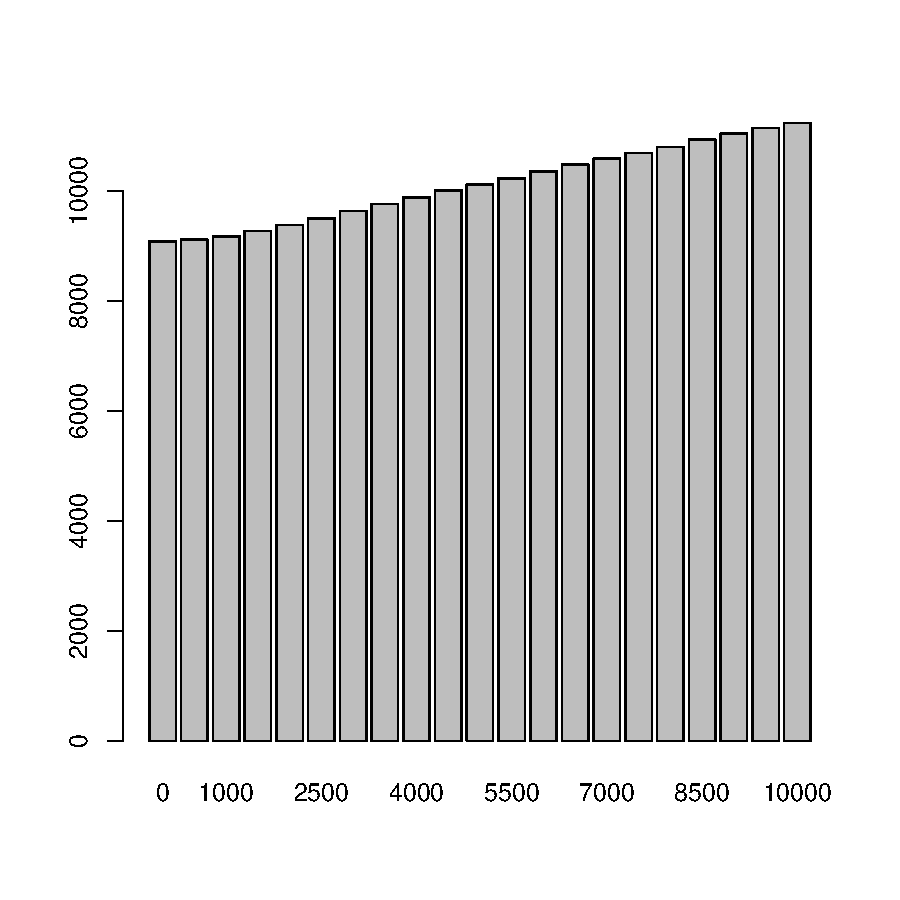
\includegraphics{geneXtendeR-015}
\end{center}
\end{figure}

This command first generates 21 individual whole-genome files: 0, 500, 1000, ..., and 10000 bp upstream extension files for the rat (\emph{Rattus norvegicus}) genome, each having an automatic 500 bp downstream extension.  In other words, each gene in the rat genome is extended upstream and downstream by some user-specified distance, thereby creating a ``gene-sphere."  As such, this bar chart command visualizes the raw count of the number of peaks that are sitting on top of genes at each individual upstream cutoff.  Clearly, the wider the gene-sphere, the more peaks-on-top-of-genes are found throughout the genome.  However, the law of diminishing returns begins to kick in at increasing upstream extension levels (see \texttt{linePlot()} for a visual representation):

\begin{figure}[H]
\begin{center}
\begin{Schunk}
\begin{Sinput}
> linePlot(rat, 0, 10000, 500)
\end{Sinput}
\end{Schunk}
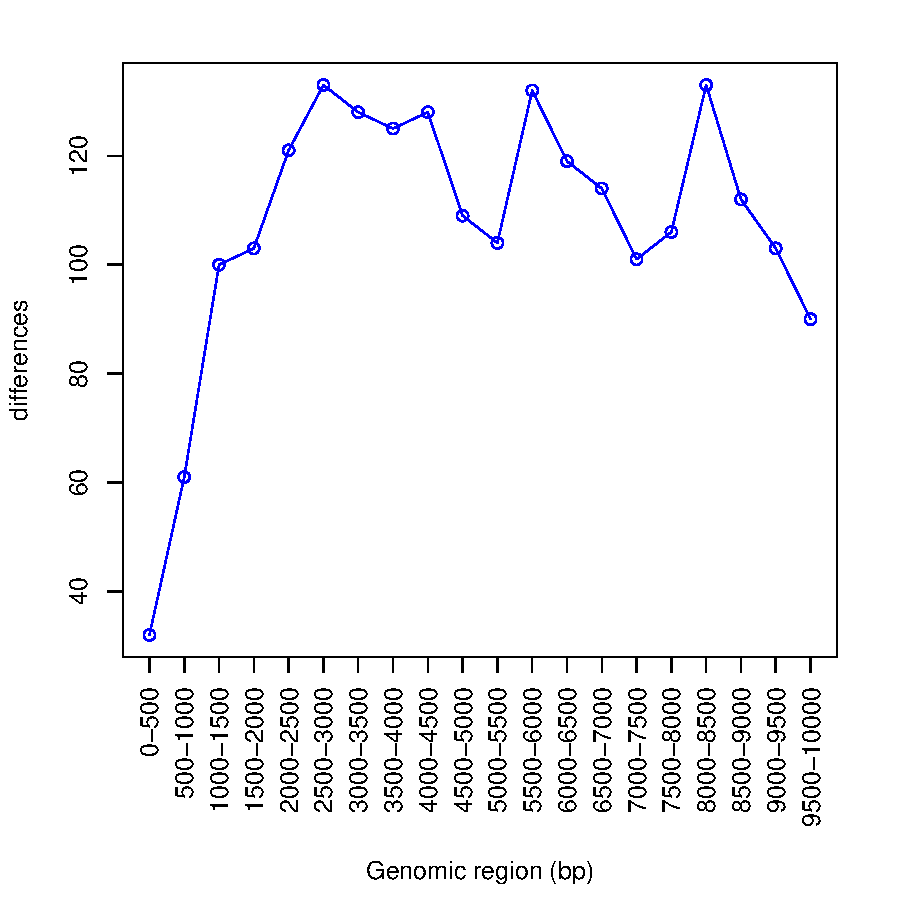
\includegraphics{geneXtendeR-016}
\end{center}
\end{figure}

In this line plot, there is a sharp rise in the number of peaks-on-top-of-genes from a 0 bp upstream extension to a 1500 bp upstream extension, and from a 2000 bp upstream extension to a 3000 bp upstream extension.  This steady rise up until 3000 bp is followed by a steady decline at subsequent extension levels followed by some noisy fluctuations.  It may be interesting to investigate what is going on in the interval from 2000 bp to 3000 bp: 

\begin{figure}[H]
\begin{center}
\begin{Schunk}
\begin{Sinput}
> linePlot(rat, 2000, 3000, 100)
\end{Sinput}
\end{Schunk}
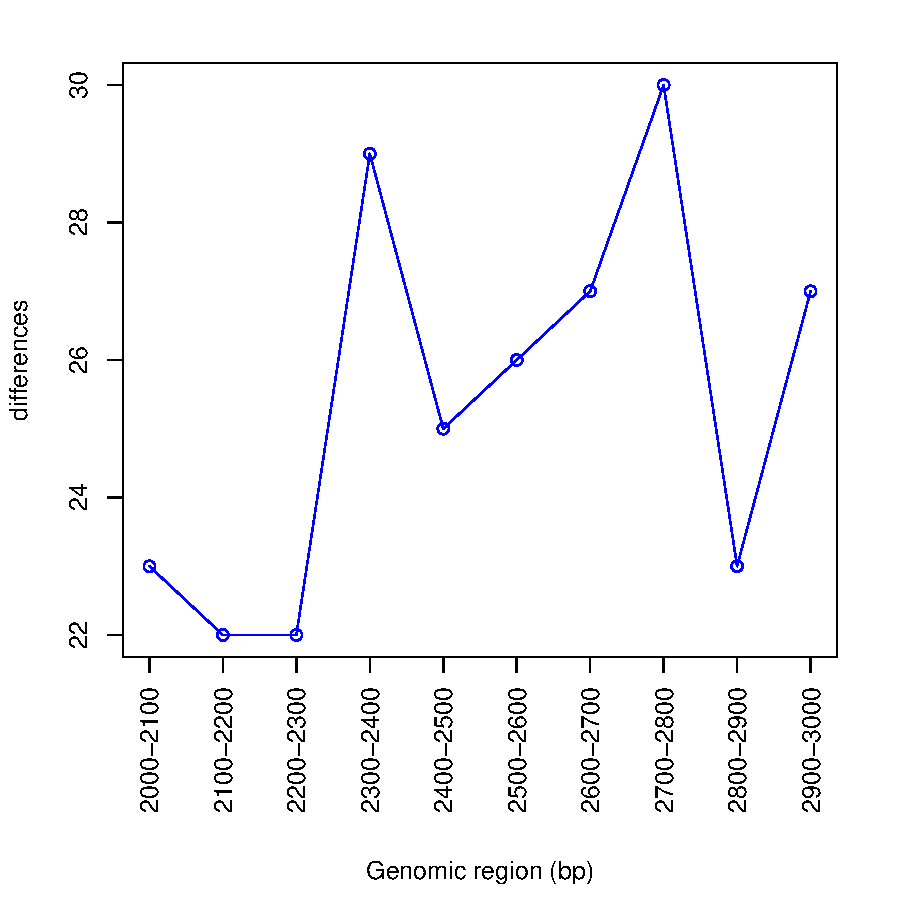
\includegraphics{geneXtendeR-017}
\end{center}
\end{figure}

Visually, there is a relative spike in the number of peaks-on-top-of-genes at the 2400 bp upstream extension (as compared to the 2300 bp extension).  This spike then drops back down at subsequent extension levels and fluctuates in a noisy manner.  However, a cumulative line plot shows that this ``spike" is more of a visual effect than anything else, since the graph is almost perfectly linear:

\begin{figure}[H]
\begin{center}
\begin{Schunk}
\begin{Sinput}
> cumlinePlot(rat, 2000, 3000, 100)
\end{Sinput}
\end{Schunk}
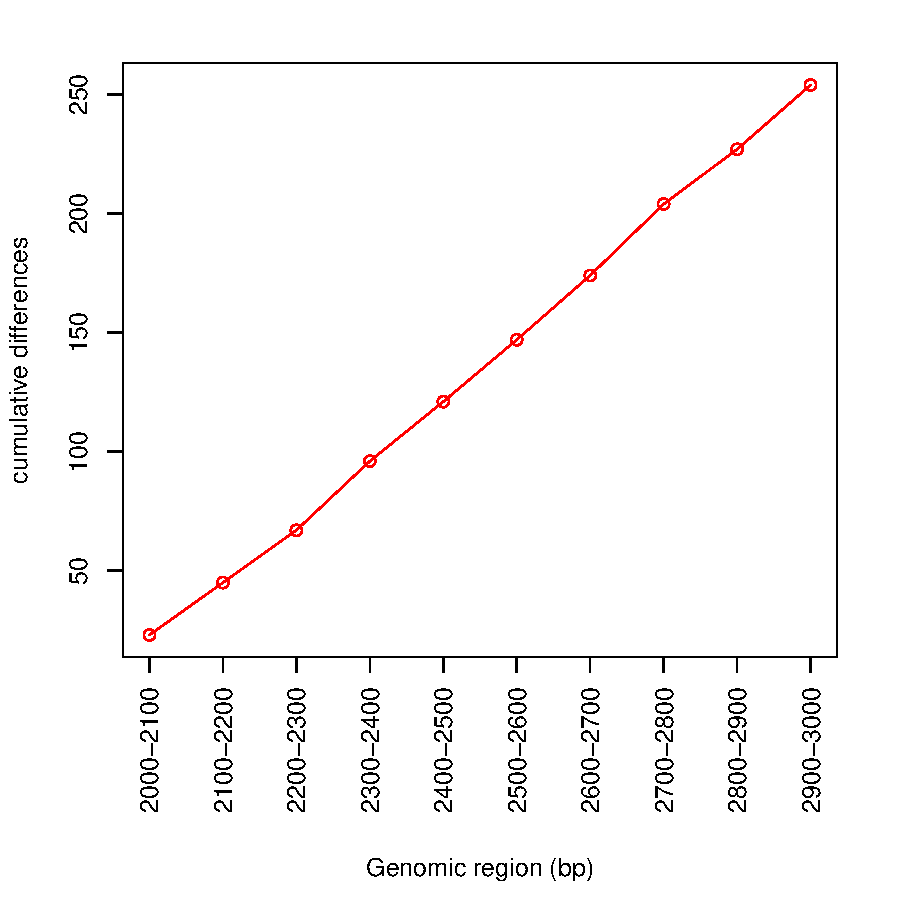
\includegraphics{geneXtendeR-018}
\end{center}
\end{figure}

Hence, one very useful function in \texttt{geneXtendeR} is called \texttt{hotspotPlot()}, which allows users to examine the ratio of statistically significant peaks\footnote{Note that statistical significance is set apriori by the user at the peak calling stage (prior to \texttt{geneXtendeR}) to give the user the freedom to choose how to filter out peak coordinates that only pass specific p-value and FDR cutoffs from a peak caller.  Peak caller output (e.g., from SICER) gives both p-value and FDR measures for each peak, thereby making it easy to extract only the peak coordinates that pass a specific set of statistical cutoff criteria.} to the total number of peaks at each genomic interval (e.g., 0-500 bp upstream of every gene in the genome, 500-1000 bp upstream of every gene in the genome, etc.). 

\begin{figure}[H]
\begin{center}
\begin{Schunk}
\begin{Sinput}
> allpeaks <- system.file("extdata", "totalpeaksfile.txt", 
+                         package="geneXtendeR")
> sigpeaks <- system.file("extdata", 
+                         "significantpeaksfile.txt",
+                         package="geneXtendeR")
> hotspotPlot(allpeaks, sigpeaks, rat, 0, 10000, 500)
\end{Sinput}
\end{Schunk}
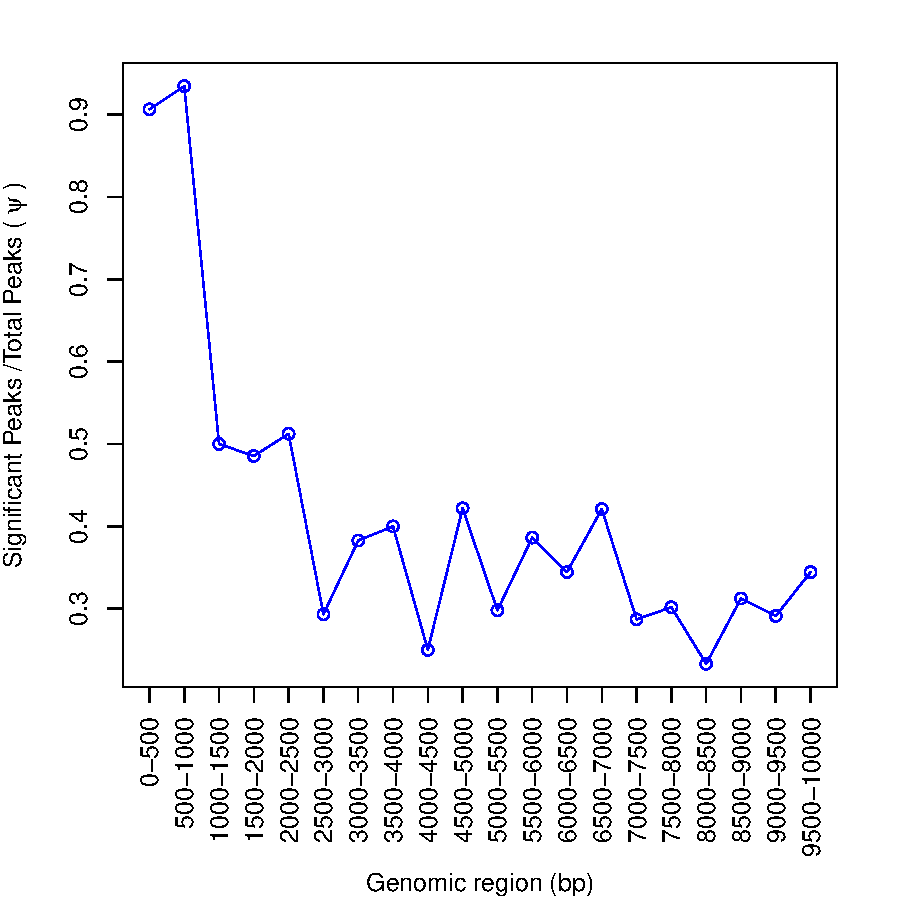
\includegraphics{geneXtendeR-019}
\end{center}
\end{figure}

This line plot shows that the concentration of significant peaks in this dataset (Barbier et al. 2016) is highest between 0 and 1000 bp upstream of a gene, with over 90\% of peaks in these regions being statistically significant.  In contrast, between 1000 bp and 2500 bp, only about half of the total peaks contained in these intervals are significant.  Statistical significance then fluctuates noisly at further upstream genomic intervals, but with at least a quarter (25\%) of the total peaks in these further upstream regions being statistically significant.  As such, the take-home message is that genomic regions within the first 1000 bp upstream of their respective genes are most likely to contain significant peaks (relative to the total peak count in these regions) and are therefore hotspots, but regions beyond this also contain a fair share of statistically significant peaks.

One interesting area to investigate is the variance in the broadness of significant (or total) peaks across different genomic intervals\footnote{One can either observe the global distribution of peak lengths within specific genomic intervals (see \texttt{?peakLengthBoxplot()}), or observe the global distribution of peak lengths across all intervals (see \texttt{?allPeakLengths()}).}.  In other words, asking questions like ``are statistically significant peaks that are located very close to their nearest gene (e.g., 0-500 bp away) wider or narrower than peaks located 500-1000 bp away from their nearest gene?".  To answer this question we can do:

\begin{figure}[H]
\begin{center}
\begin{Schunk}
\begin{Sinput}
> sigpeaks <- system.file("extdata", 
+                         "significantpeaksfile.txt",
+                         package="geneXtendeR")
> peaksInput(sigpeaks)
> meanPeakLengthPlot(rat, 0, 10000, 500)
\end{Sinput}
\end{Schunk}
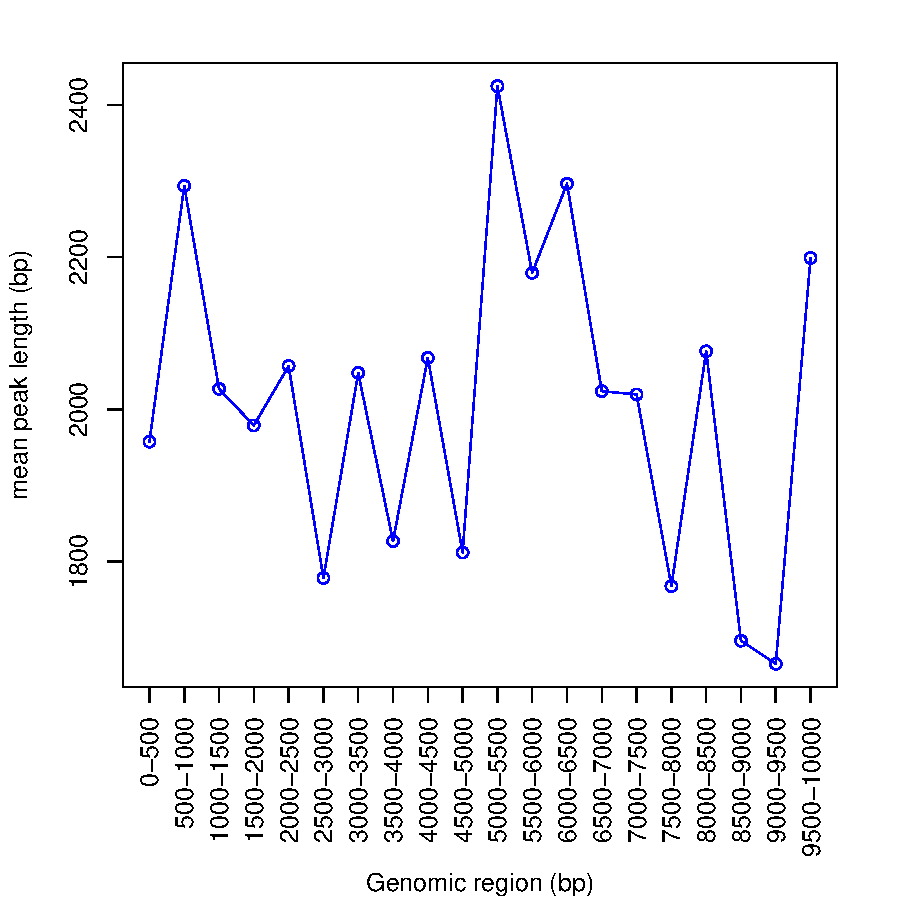
\includegraphics{geneXtendeR-020}
\end{center}
\end{figure}

This line plot displays the mean (average) length of all significant peaks found within each genomic interval.  Clearly, the ``average peak" is slightly narrower in 0-500 bp intervals than in 500-1000 bp intervals yet, overall, peak lengths tend to fluctuate more or less stochastically at various intervals.  To get the exact peak length, we can do:

\begin{Schunk}
\begin{Sinput}
> sigpeaks <- system.file("extdata", "significantpeaksfile.txt",
+                         package="geneXtendeR")
> peaksInput(sigpeaks)
> meanPeakLength(rat, 0, 500)
\end{Sinput}
\begin{Soutput}
[1] 1957.621
\end{Soutput}
\end{Schunk}

So the mean peak length in the interval 0-500 bp is approximately 1958 bp.  Although we see that there is no specific interval with peaks of extraordinary average lengths, it is still possible to see peak length outliers in certain cases (especially when looking at total peak sets):  

\begin{figure}[H]
\begin{center}
\begin{Schunk}
\begin{Sinput}
> allpeaks <- system.file("extdata", "totalpeaksfile.txt",
+                         package="geneXtendeR")
> peaksInput(allpeaks)
> meanPeakLengthPlot(rat, 0, 10000, 500)
\end{Sinput}
\end{Schunk}
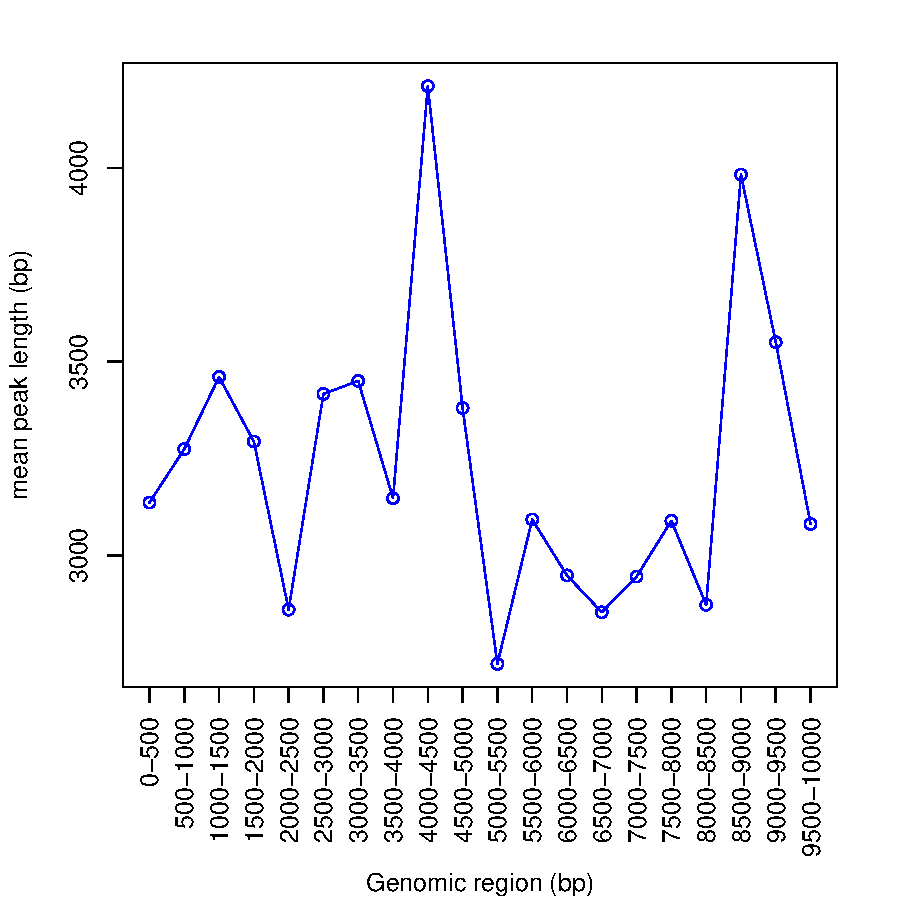
\includegraphics{geneXtendeR-022}
\end{center}
\end{figure}

We see that the 4000-4500 bp and 8500-9000 bp intervals both look quite different in terms of their mean peak lengths relative to the other intervals.  To see if the mean might be influenced by a strong outlier(s), we can do:

\begin{figure}[H]
\begin{center}
\begin{Schunk}
\begin{Sinput}
> allpeaks <- system.file("extdata", "totalpeaksfile.txt",
+                         package="geneXtendeR")
> peaksInput(allpeaks)
> peak_lengths <- peakLengthBoxplot(rat, 4000, 4500)
\end{Sinput}
\end{Schunk}
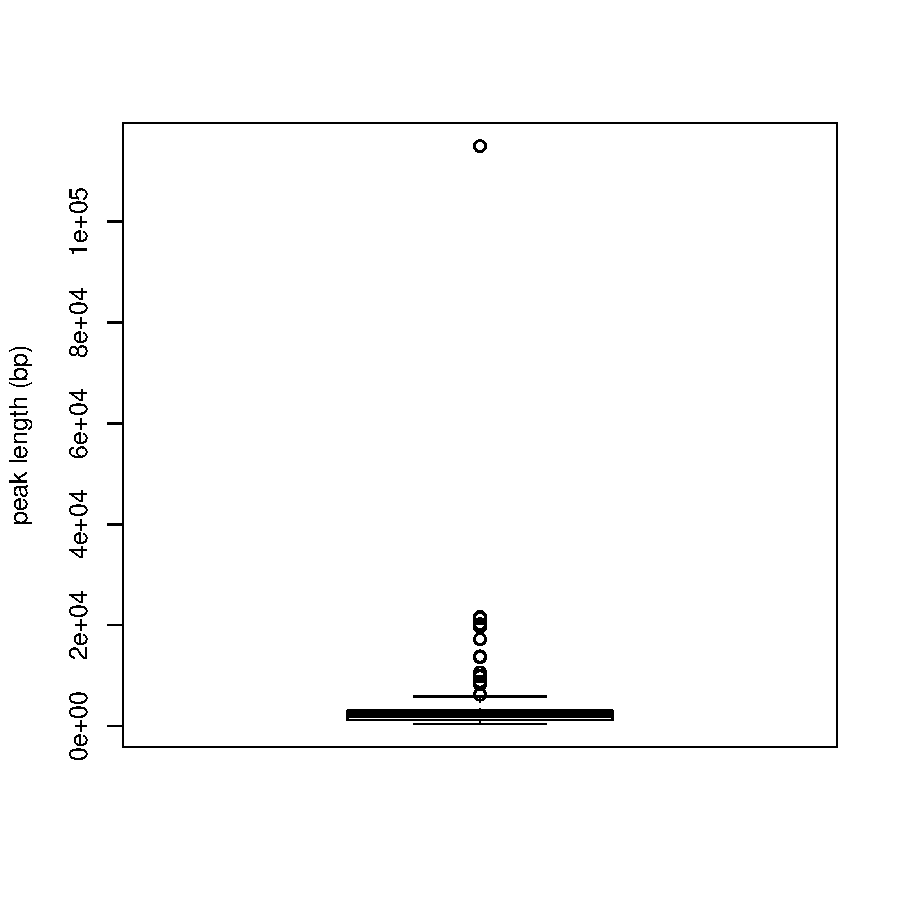
\includegraphics{geneXtendeR-023}
\end{center}
\end{figure}

This box-and-whisker plot shows a clear outlier, which is an example of a very broad peak.  We can find the exact length of this outlier peak using: 

\begin{Schunk}
\begin{Sinput}
> peak_lengths <- peakLengthBoxplot(rat, 4000, 4500)
> max(peak_lengths)
\end{Sinput}
\begin{Soutput}
[1] 114999
\end{Soutput}
\end{Schunk}

So this outlier peak measures 114999 bp in total length, therefore making it an extremely broad peak.  To see what nearest gene it resides to, we can first extract the peak's index by:

\begin{Schunk}
\begin{Sinput}
> peak_lengths <- peakLengthBoxplot(rat, 4000, 4500)
> match(114999, peak_lengths)
\end{Sinput}
\begin{Soutput}
[1] 126
\end{Soutput}
\end{Schunk}

which returns the index of where this peak length is found.  Then the following command finds all unique peaks that reside between 4000 and 4500 bp upstream of their nearest gene:

\begin{Schunk}
\begin{Sinput}
> distinct(rat, 4000, 4500)
\end{Sinput}
\begin{Soutput}
     Chromosome Peak-Start  Peak-End Gene-Chr Gene-Start  Gene-End
  1:          1   19526200  19526799        1   19520708  19526671
  2:          1   61630800  61631999        1   61624941  61630954
  3:          1   71346800  71347999        1   71334629  71347133
  4:          1   98385400  98394199        1   98394160  98403468
  5:          1  101099600 101101399        1  101086377 101100094
 ---                                                              
124:         18   60006800  60007199       18   59985860  60007069
125:         19   45499400  45499799       19   45499420  45507827
126:         19   54877400  54992399       19   54871853  54877469
127:         20   30610800  30620799       20   30606026  30611101
128:        100   73017400  73018799      100   73018667  73024598
                Gene-ID      Gene-Name Distance
  1: ENSRNOG00000030796 AABR07000595.1        0
  2: ENSRNOG00000025949        Vom1r22        0
  3: ENSRNOG00000049014   LOC100912263        0
  4: ENSRNOG00000037331           Cd33        0
  5: ENSRNOG00000020583          Fcgrt        0
 ---                                           
124: ENSRNOG00000017852           Nars        0
125: ENSRNOG00000053551 AABR07043877.1        0
126: ENSRNOG00000028578 AABR07044065.1        0
127: ENSRNOG00000049167 AABR07044988.1        0
128: ENSRNOG00000027980 AABR07039245.1        0
\end{Soutput}
\end{Schunk}

where we see that index \texttt{126} belongs to gene \texttt{AABR07044065.1}\footnote{This peak may not be statistically significant, but how could it be if it's so huge?  In situations like this, it may be a good idea to check what is known about the gene already: \url{http://www.pantherdb.org/genes/gene.do?acc=RAT\%7CEnsembl\%3DENSRNOG00000028578\%7CUniProtKB\%3DA0A0G2K0W2}.  Clearly, not much is known yet.}.  Checking the arithmetic difference between column 3 and column 2 for this specific row verifies 114999, as these two columns represent the peak start position and peak end positions.  Now let's identify what the other columns represent by running the \texttt{distinct()} function again (but this time on a smaller interval to have less output printed to the screen):    

\begin{Schunk}
\begin{Sinput}
> fpath <- system.file("extdata", "somepeaksfile.txt", 
+                      package="geneXtendeR")
> peaksInput(fpath)
> distinct(rat, 2300, 2400)
\end{Sinput}
\begin{Soutput}
    Chromosome Peak-Start  Peak-End Gene-Chr Gene-Start  Gene-End
 1:          1   79718600  79725199        1   79725197  79728613
 2:          1  188715600 188716999        1  188688243 188715680
 3:          1  214368800 214373199        1  214373115 214386385
 4:          1  221669800 221671199        1  221671190 221694018
 5:          1  236532800 236534799        1  236529431 236532885
 6:          3   82239000  82242199        3   82096568  82239064
 7:          3   82780200  82784599        3   82762362  82780214
 8:          3  146409600 146412399        3  146376328 146409652
 9:          3  165702800 165706799        3  165678807 165702889
10:          4   84850400  84851999        4   84851986  84872257
11:          4  118157000 118157799        4  118157747 118166562
12:          4  171955800 171956999        4  171956961 171961084
13:          4  180237200 180239199        4  180231882 180237204
14:          5   36437600  36438199        5   36433358  36437694
15:          5   69038200  69039399        5   69035218  69038218
16:          5  121456000 121457199        5  121451803 121456072
17:          5  153628200 153630199        5  153568245 153628269
18:          7   14586000  14587199        7   14587120  14615369
19:          7   75225000  75225799        7   75225775  75249569
20:          8  133130600 133133199        8  133126720 133130690
21:         10    1830200   1832199       10    1832118   1841132
22:         11   80315400  80316799       11   80316777  80332099
23:         14   76654000  76654999       14   76654911  76833661
24:         14  103716400 103719199       14  103711769 103716440
25:         16     631200    642399       16     517332    631224
26:         16    9020200   9020999       16    9020987   9055164
27:         16   75363800  75364599       16   75364529  75368406
28:         20    1747000   1747399       20    1747316   1751142
29:         20   22423400  22426199       20   22420251  22423425
    Chromosome Peak-Start  Peak-End Gene-Chr Gene-Start  Gene-End
               Gene-ID      Gene-Name Distance
 1: ENSRNOG00000026891     AC093995.1        0
 2: ENSRNOG00000016013         Gprc5b        0
 3: ENSRNOG00000018367         Taldo1        0
 4: ENSRNOG00000027456       Cdc42bpg        0
 5: ENSRNOG00000022308   LOC103691298        0
 6: ENSRNOG00000008758        Tspan18        0
 7: ENSRNOG00000042533          Accsl        0
 8: ENSRNOG00000006795          Apmap        0
 9: ENSRNOG00000042101          Zfp93        0
10: ENSRNOG00000010205          Mturn        0
11: ENSRNOG00000016273        Fam136a        0
12: ENSRNOG00000057540 AABR07062363.1        0
13: ENSRNOG00000048961        Bhlhe41        0
14: ENSRNOG00000055329 AABR07047528.1        0
15: ENSRNOG00000060997             U6        0
16: ENSRNOG00000045614   LOC102552337        0
17: ENSRNOG00000018109          Clic4        0
18: ENSRNOG00000048450        Cyp4f37        0
19: ENSRNOG00000061463 AABR07057510.3        0
20: ENSRNOG00000006730         Ccr1l1        0
21: ENSRNOG00000040121     RGD1565158        0
22: ENSRNOG00000022160           Rtp2        0
23: ENSRNOG00000051169           Clnk        0
24: ENSRNOG00000054704 AABR07016558.1        0
25: ENSRNOG00000061982 AABR07024473.2        0
26: ENSRNOG00000042628     RGD1561145        0
27: ENSRNOG00000029462         Defal1        0
28: ENSRNOG00000050043        Olr1735        0
29: ENSRNOG00000057124 AABR07044824.1        0
               Gene-ID      Gene-Name Distance
\end{Soutput}
\end{Schunk}

This data table shows 29 separate entries sorted by chromosome and start position.  \texttt{Gene-ID} refers to the Ensembl ID and the other columns named accordingly. It should be noted that the X chromosome is designated by the integer 100, the Y chromosome by the integer 200, and the mitochondrial chromosome by the integer 300.  This is done for sorting purposes (see \texttt{?peaksInput} for details).  In short, the \texttt{distinct()} command finds what peaks-on-top-of-genes would be missed if a 2300 bp upstream extension is used instead of a 2400 bp extension.  In other words, these 29 genes all reside between 2300-2400 bp upstream of their nearest gene.

Once the user has chosen the specific upstream extension to be used, the peak file is ready to be fully annotated:

\begin{Schunk}
\begin{Sinput}
> annotate(rat, 2400)
\end{Sinput}
\begin{Soutput}
       Chromosome Peak-Start  Peak-End Gene-Start  Gene-End            Gene-ID
    1:          1      48800     51199     394300    410176 ENSRNOG00000046319
    2:          1      53000     53799     394300    410176 ENSRNOG00000046319
    3:          1     265600    266999     394300    410176 ENSRNOG00000046319
    4:          1     506600    507999     394300    410176 ENSRNOG00000046319
    5:          1     669400    672199     697013    708565 ENSRNOG00000047964
   ---                                                                        
25085:        100  159818600 159820599  159723366 159843472 ENSRNOG00000000869
25086:        100  159821400 159823199  159723366 159843472 ENSRNOG00000000869
25087:        100  159898400 159899599  159889343 159892315 ENSRNOG00000054559
25088:        100  159913800 159915199  159889343 159892315 ENSRNOG00000054559
25089:        100  159947000 159948599  159889343 159892315 ENSRNOG00000054559
          Gene-Name Distance-of-Gene-to-Nearest-Peak
    1:       Vom2r3                           361377
    2:       Vom2r3                           357177
    3:       Vom2r3                           144577
    4:       Vom2r3                            96425
    5: LOC100909608                            24815
   ---                                              
25085:      Arhgef6                                0
25086:      Arhgef6                                0
25087:      SNORD61                             6086
25088:      SNORD61                            21486
25089:      SNORD61                            54686
\end{Soutput}
\end{Schunk}

which generates a fully annotated peaks outfile (in the user's working directory) containing various genomic features and labeled headers. An example of which is above.

\subsection{Exploring functional annotation in depth}

If a user is looking for a more gene-centric approach to an\-notation (as briefly outlined in Section \ref{sec:centric}), they may use either the \texttt{gene\_lookup()}
or \texttt{gene\_annotate()} functions. The \texttt{gene\_annotate()} function builds off of the \texttt{annotate()} function, but reorganizes and groups the output based on relevant gene information.  If you (the reader) are just joining us now in the vignette and have not yet run any of the command on preceding pages, first just run the following commands:

\begin{Schunk}
\begin{Sinput}
> library(geneXtendeR)
> rat <- readGFF("ftp://ftp.ensembl.org/pub/release-84/gtf/
+                       rattus_norvegicus/
+                       Rattus_norvegicus.Rnor_6.0.84.chr.gtf.gz")
> fpath <- system.file("extdata", "somepeaksfile.txt", 
+                      package="geneXtendeR")
> peaksInput(fpath)
\end{Sinput}
\end{Schunk}

Now do:

\begin{Schunk}
\begin{Sinput}
> head(gene_annotate(rat, 2400))
\end{Sinput}
\begin{Soutput}
  Chromosome Gene-Start  Gene-End            Gene-ID Gene-Name
1         12   14448510  15101186 ENSRNOG00000001103      Sdk1
2          5  168141047 168736696 ENSRNOG00000018602    Camta1
3          8  127268889 127573488 ENSRNOG00000043167     Itga9
4         13  106749225 107427829 ENSRNOG00000003738     Ush2a
5         10   18557628  18944940 ENSRNOG00000005365    Kcnip1
6         12   51385263  51705130 ENSRNOG00000032590     Ttc28
  Peaks-on-Gene-Body Mean-Distance-of-Gene-to-Nearest-Peaks       sd
1                 32                               6290.222 19899.71
2                 21                                  0.000     0.00
3                 20                                  0.000     0.00
4                 20                                  0.000     0.00
5                 19                                  0.000     0.00
6                 19                                  0.000     0.00
  Number-of-Peaks-Associated-with-Gene
1                                   36
2                                   21
3                                   20
4                                   20
5                                   19
6                                   19
\end{Soutput}
\end{Schunk}

This output labels each gene and matches it with the number of peaks that overlap it and are "first away" from its gene-body (i.e., closest/nearest but not overlapping).  Distance is calculated between 5-prime end of gene and 3-prime end of peak (or 3-prime end of gene and 5-prime end of peak, whichever is smallest).  The table is sorted by number of peaks on gene body (i.e., number of peaks that directly overlap the gene body) and include extra information such as mean and standard deviation (sd) for extra validation.  Typically, a user would be looking for genes that have a high number of \texttt{Peaks-on-Gene-Body} to follow-up on for experimental validation. Genes that have peaks that reside close (but not overlapping) to the chosen gene-body (i.e., low mean) and that are clustered together spatially (i.e., low standard deviation) may also be good targets for follow-up analysis. 


An example of how the \texttt{gene\_annotate()} function is intended to be used is below, where we highlight three specific rows to highlight key points of the discussion:

\begin{Schunk}
\begin{Sinput}
> gene_annotate(rat, 2400)[c(1, 7, 11),]
\end{Sinput}
\begin{Soutput}
   Chromosome Gene-Start Gene-End            Gene-ID Gene-Name
1          12   14448510 15101186 ENSRNOG00000001103      Sdk1
7           8   52984813 53149353 ENSRNOG00000029980    Zbtb16
11         19   20144637 20406503 ENSRNOG00000014658    Zfp423
   Peaks-on-Gene-Body Mean-Distance-of-Gene-to-Nearest-Peaks        sd
1                  32                              6290.2222 19899.710
7                  17                               740.1579  2336.913
11                 13                             19803.6500 33367.643
   Number-of-Peaks-Associated-with-Gene
1                                    36
7                                    19
11                                   20
\end{Soutput}
\end{Schunk}

These three genes exemplify three of the four different scenarios that may occur in this table. The difference between the mean and the standard deviation of the peaks located closest to a specific gene can be used to judge the distribution of those peaks, thereby indicating what may or may not be worth following up on in the wet-lab experiments.
\begin{enumerate}
\item The first gene has 32 peaks on the gene-body of "Sdk1" (i.e., 32 peaks that overlap a 2400 bp upstream and 500 bp downstream extension of "Sdk1"), with a total of 36 genes annotated to the "Sdk1" gene body in total. The high SD and mean (relative to the fact that 32/36 of these genes reside on the gene-body itself) indicate that the other 4 peaks that do not reside on gene-body, also do not reside near enough to the gene to warrant biological meaning. In other words, focus on the 32 peaks on the gene-body itself and not the other 4.
\item The second gene has both a low mean distance as well as a relatively low standard deviation, which indicates that peaks not residing on the extended gene-body are still quite close to it and clustered together spatially at approximately the same genomic location (possibly a proximal-promoter region).  "Zbtb16" is definitely a good gene to follow-up on because the peaks are close enough to the gene body to be considered biologically important (e.g., might reside in important proximal-promoter regions of the gene).
\item The third gene showcases the default case, in which both the mean and sd are relatively high. The peaks that do not reside on "Zfp423" are not close or clustered together either, based on the spread of the mean and standard deviation, so the 7 additional peaks are probably unnecessary for use in a follow-up of that gene.  The reason why the \texttt{geneXtendeR} package registers these 7 peaks in the first place (even though their mean distance is 19804 bp from their nearest genes) is because these peaks are located in intergenic regions where "Zfp423" just so happens to be the closest gene.
\item The final case is the rarest case, when the mean is high but the standard deviation is low. This indicates that the peaks are grouped, but located far away from the closest gene-body. This may be another case worth following up on, especially in the context of long-range interactions (e.g., trans-regulatory elements).
\end{enumerate}

It should be noted that mean = 0 (i.e, \texttt{Mean-Distance-of-Gene-to-Nearest-Peaks} = 0) denotes cases where all peaks are overlapping a given gene body.  

The \texttt{gene\_lookup()} function looks up all peaks surrounding a specific gene or list of genes across all chromosomes and reports these peaks. This method is extremely useful when paired with \texttt{gene\_annotate()} to check genes that may be used in a follow-up.

\begin{Schunk}
\begin{Sinput}
> gene_lookup(rat, c("Zbtb16"), n = 19, extension = 2400)
\end{Sinput}
\begin{Soutput}
    Chromosome Peak-Start Peak-End Distance-to-Gene Gene-Start Gene-End   Gene
 1:          8   52983400 52986999                0   52984813 53149353 Zbtb16
 2:          8   52988000 52988999                0   52984813 53149353 Zbtb16
 3:          8   52989600 52992199                0   52984813 53149353 Zbtb16
 4:          8   52993000 52995799                0   52984813 53149353 Zbtb16
 5:          8   52998400 53004399                0   52984813 53149353 Zbtb16
 6:          8   53006200 53009399                0   52984813 53149353 Zbtb16
 7:          8   53024400 53031999                0   52984813 53149353 Zbtb16
 8:          8   53038200 53040799                0   52984813 53149353 Zbtb16
 9:          8   53044000 53046399                0   52984813 53149353 Zbtb16
10:          8   53084800 53085799                0   52984813 53149353 Zbtb16
11:          8   53090800 53094999                0   52984813 53149353 Zbtb16
12:          8   53096200 53099999                0   52984813 53149353 Zbtb16
13:          8   53101000 53105799                0   52984813 53149353 Zbtb16
14:          8   53106600 53110399                0   52984813 53149353 Zbtb16
15:          8   53119600 53132199                0   52984813 53149353 Zbtb16
16:          8   53132800 53135799                0   52984813 53149353 Zbtb16
17:          8   53138000 53152999                0   52984813 53149353 Zbtb16
18:          8   52946600 52979999             4814   52984813 53149353 Zbtb16
19:          8   53158600 53163799             9247   52984813 53149353 Zbtb16
\end{Soutput}
\end{Schunk}

This output shows all the peaks nearest to "Zbtb16" and their respective distances.  Knowing these genomic peak coordinates facilitates the design of PCR primers.  Although 17/19 of the peaks reside on the extended gene-body (2400 bp upstream extension, 500 bp downstream extension), the two additional peaks are still close enough to be considered for analysis.  Out of all the genes on that specific chromosome, these two nearby peaks are located closest to the gene "Zbtb16".

In \texttt{gene\_lookup(organism, gene\_name, n, extension)}, n represents the number of nearest (and overlapping) peaks to a given gene. We saw from \texttt{gene\_annotate()} that, in the case of "Zbtb16," there are 19 nearest (and overlapping) peaks to the gene and \texttt{gene\_lookup()} displays their location as well as their distance from the gene. This function is motivated by the need of biologists to accurately design primers for specific genomic loci in order to experimentally validate the existence (realness) of a peak.

For a much more in-depth analysis, a function that combines both \texttt{gene\_lookup()} and \texttt{gene\_annotate()} has been provided as \texttt{annotate\_n()}. Instead of simply annotating a peak to a single closest gene (and reporting any overlapping peaks on gene bodies), this function annotates each peak to the closest, the second-closest, ..., to the nth-closest genes to provide the user an expanded picture of the peaks layout for further analysis. Called, this function looks like:

\begin{Schunk}
\begin{Sinput}
> annotate_n(rat, 3500, n = 3)
\end{Sinput}
\begin{Soutput}
       Peak-Num Chromosome Peak-Start  Peak-End Gene-Start  Gene-End
    1:        1          1      48800     51199     393200    410176
    2:        1          1      48800     51199     695913    708565
    3:        1          1      48800     51199     744116    759145
    4:        2          1      53000     53799     393200    410176
    5:        2          1      53000     53799     695913    708565
   ---                                                              
75263:    25088        100  159913800 159915199  159889343 159893415
75264:    25088        100  159913800 159915199  159723366 159844572
75265:    25089        100  159947000 159948599  159884385 159894826
75266:    25089        100  159947000 159948599  159889343 159893415
75267:    25089        100  159947000 159948599  159723366 159844572
                  Gene-ID    Gene-Name rank Minimum-Distance-to-Gene
    1: ENSRNOG00000046319       Vom2r3    1                   342001
    2: ENSRNOG00000047964 LOC100909608    2                   644714
    3: ENSRNOG00000050370       Vom2r6    3                   692917
    4: ENSRNOG00000046319       Vom2r3    1                   339401
    5: ENSRNOG00000047964 LOC100909608    2                   642114
   ---                                                              
75263: ENSRNOG00000054559      SNORD61    2                    20385
75264: ENSRNOG00000000869      Arhgef6    3                    69228
75265: ENSRNOG00000000866         Rbmx    1                    52174
75266: ENSRNOG00000054559      SNORD61    2                    53585
75267: ENSRNOG00000000869      Arhgef6    3                   102428
\end{Soutput}
\end{Schunk}

This function is the most versatile of the annotation functions provided and is designed for the purpose of providing peak-to-gene associations and follow-up information that goes beyond just a simple closest genomic distance criterion.  Future work in this direction can address three-dimensional genome interactions (when coupled with methods like Hi-C).  When moving away from the traditional "first closest gene" to a peak, this method opens up many more possibilities as to which peaks influence which genes. It increases the scope of the individual peaks to reduce the chance that a peak that influences any particular gene is missed or misattributed to the wrong gene.

\subsection{Gene Ontology functions} \label{sec:GO}

It may be of interest to note the differential gene ontologies between the following two upstream extensions:

\begin{Schunk}
\begin{Sinput}
> library(org.Rn.eg.db)
> library(GO.db)
> x <- diffGO(rat, 2300, 2400, BP, org.Rn.eg.db)
> head(x, 20)
\end{Sinput}
\begin{Soutput}
   gene$SYMBOL       GOID
1       Gprc5b GO:0001934
2       Gprc5b GO:0007186
3       Gprc5b GO:0007626
4       Gprc5b GO:0010976
5       Gprc5b GO:0032147
6       Gprc5b GO:0042593
7       Gprc5b GO:0043123
8       Gprc5b GO:0045666
9       Gprc5b GO:0045860
10      Gprc5b GO:0050729
11      Gprc5b GO:0060907
12      Gprc5b GO:0061098
13      Gprc5b GO:0090263
14      Taldo1 GO:0005975
15      Taldo1 GO:0006002
16      Taldo1 GO:0006098
17      Taldo1 GO:0009052
18      Taldo1 GO:0019682
19    Cdc42bpg GO:0006468
20    Cdc42bpg GO:0031532
                                                         TERM
1              positive regulation of protein phosphorylation
2                G-protein coupled receptor signaling pathway
3                                         locomotory behavior
4        positive regulation of neuron projection development
5                       activation of protein kinase activity
6                                         glucose homeostasis
7  positive regulation of I-kappaB kinase/NF-kappaB signaling
8               positive regulation of neuron differentiation
9              positive regulation of protein kinase activity
10               positive regulation of inflammatory response
11      positive regulation of macrophage cytokine production
12    positive regulation of protein tyrosine kinase activity
13     positive regulation of canonical Wnt signaling pathway
14                             carbohydrate metabolic process
15                     fructose 6-phosphate metabolic process
16                                    pentose-phosphate shunt
17              pentose-phosphate shunt, non-oxidative branch
18               glyceraldehyde-3-phosphate metabolic process
19                                    protein phosphorylation
20                          actin cytoskeleton reorganization
\end{Soutput}
\end{Schunk}

This dataframe shows the first 20 unique gene ontology terms, their IDs, and respective gene symbols.  Clearly, gene name \emph{Gprc5b} has several BP ontologies related explicitly to the brain, while \emph{Taldo1} does not.  Considering that the ChIP-seq peaks dataset used as input into \texttt{geneXtendeR} comes from a ChIP-seq study investigating the prefrontal cortex, this suggests that a 2400 bp extension may be more suitable for this brain dataset.  However, such decisions are left entirely to the discretion and judgment of the user in deciding the relative importance of specific genes and their respective GO terms (BP, CC, or MF) to the goals of the computational analysis (as well as plans for experimental follow-up and validation).  See Discussion section for details.  

It is also critical to note that the \texttt{diffGO()} function returns ALL known gene ontologies, NOT a gene ontology enrichment analysis (more about this in Discussion section).  The goal is to provide users with knowledge regarding all possible known roles of any given gene.  For example, by knowing that a potential gene candidate has previously been linked with known brain-related ontologies, a user may be prompted to look more closely into the relevant literature behind this gene and its implications to the biological question under study (before embarking on making a decision about its potential impact and suitability as a good candidate for experimental validation).  

Furthermore, a user may plot the differential gene ontology results as an interactive network:

\begin{Schunk}
\begin{Sinput}
> library(networkD3)
> library(org.Rn.eg.db)
> library(dplyr)
> makeNetwork(rat, 2300, 2400, BP, org.Rn.eg.db)
\end{Sinput}
\end{Schunk}

\begin{figure}[H]
\centering
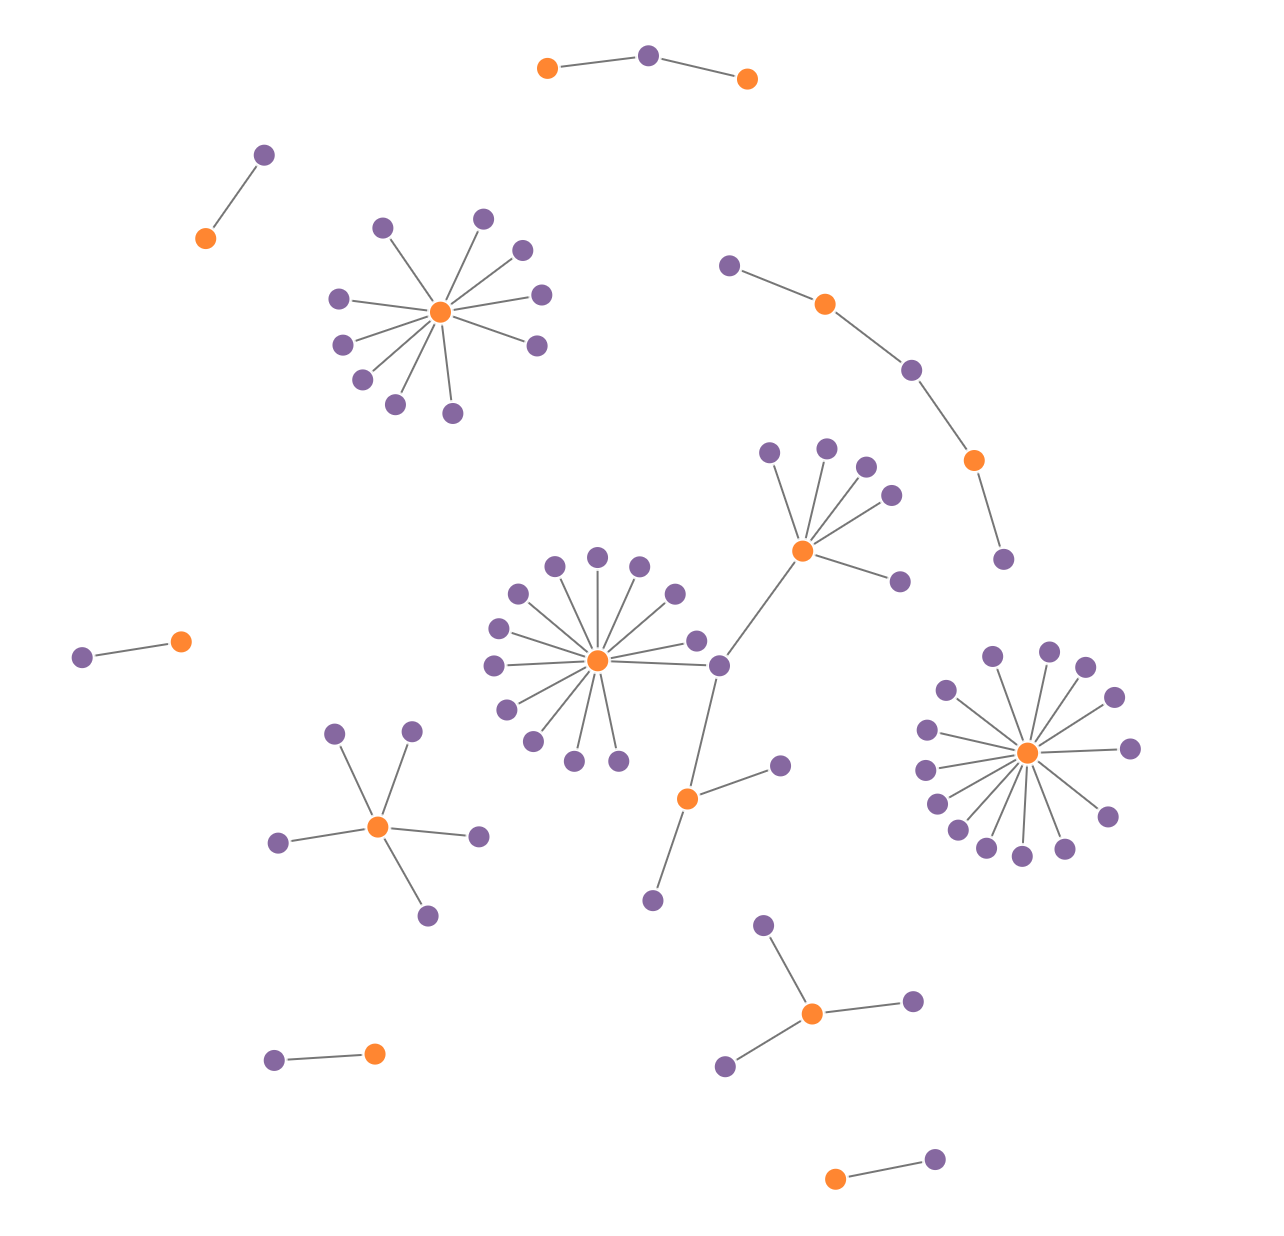
\includegraphics{figures/vignette_network_birdseye.png}
\caption{Orange color denotes gene names, purple color denotes GO terms.  A user can hover the mouse cursor over any given node to display its respective label directly within R Studio.  Likewise, users can dynamically drag and re-organize the spatial orientation of nodes, as well as zoom in and out of them for visual effect.}
\end{figure}

\begin{figure}[H]
\centering
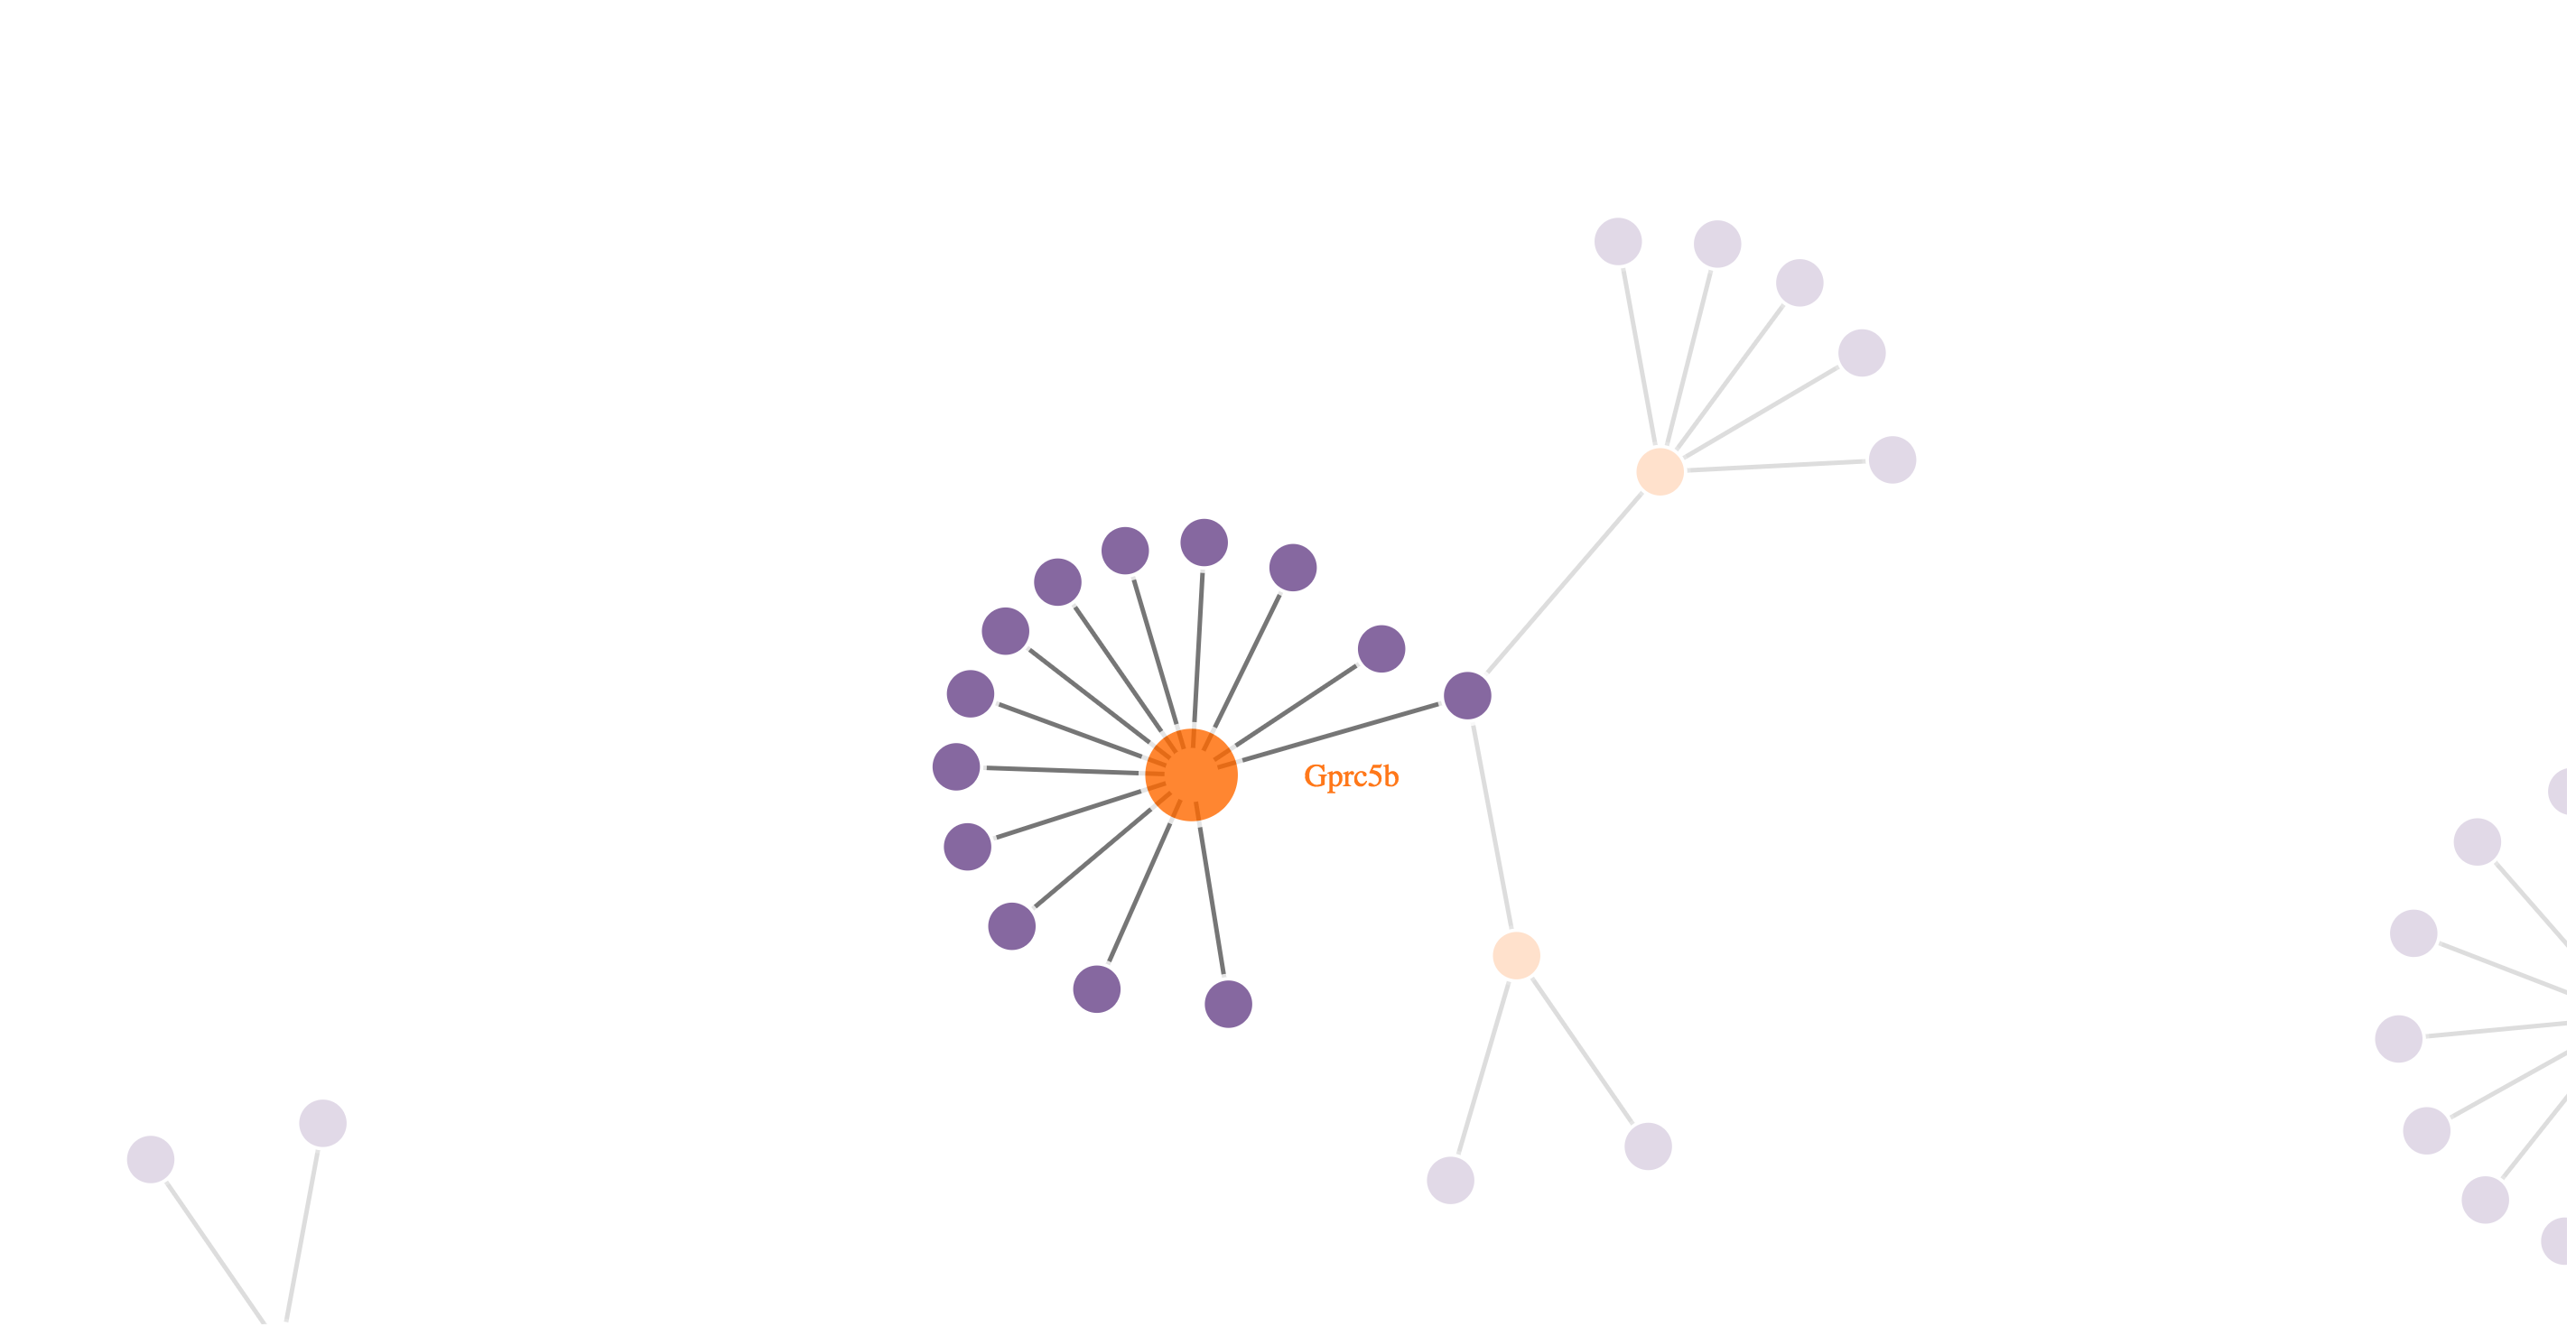
\includegraphics{figures/vignette_network_Gprc5b.png}
\caption{Orange color denotes gene names, purple color denotes GO terms.  A user can hover the mouse cursor over any given node to display its respective label directly within R Studio.  Likewise, users can dynamically drag and reorganize the spatial orientation of nodes, as well as zoom in and out of them for visual effect.}
\end{figure}

In addition, users can generate word clouds comprised from words present in their GO terms:

\begin{Schunk}
\begin{Sinput}
> library(tm)
> library(SnowballC)
> library(wordcloud)
> library(RColorBrewer)
> makeWordCloud(rat, 2300, 2400, BP, org.Rn.eg.db)
\end{Sinput}
\end{Schunk}

\begin{figure}[H]
\centering
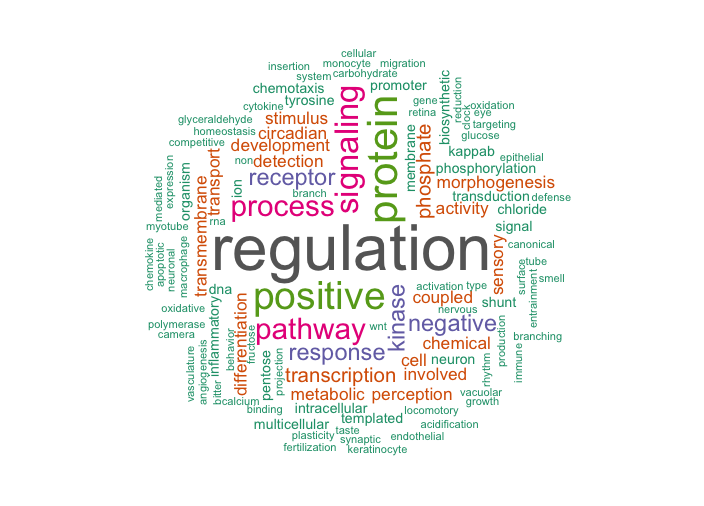
\includegraphics{figures/vignette_wordcloud.png}
\caption{Word cloud generated from words comprising gene ontology terms of category BP.  This word cloud shows the words that are used within BP gene ontology terms of peaks found to be present between 2300 and 2400 bp upstream of their nearest genes.}
\end{figure}

It may also be of interest to visually examine the most frequently used words found within GO terms:  

\begin{Schunk}
\begin{Sinput}
> library(tm)
> library(SnowballC)
> library(wordcloud)
> library(RColorBrewer)
> plotWordFreq(rat, 2300, 2400, BP, org.Rn.eg.db, 10)
\end{Sinput}
\end{Schunk}

\begin{figure}[H]
\centering
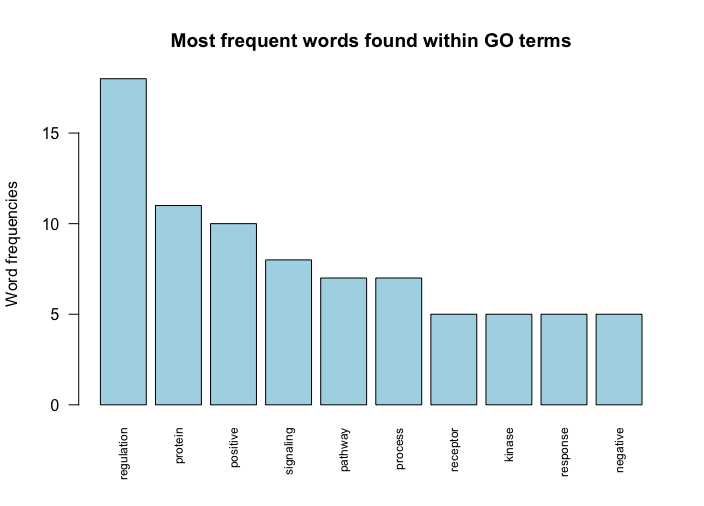
\includegraphics{figures/vignette_wordfreq.png}
\caption{This barplot shows the top 10 words used within gene ontology terms (specific to BP) of peaks found to be present between 2300 and 2400 bp upstream of their nearest genes.}
\end{figure}

\section{Discussion}

Even though \texttt{geneXtendeR} is designed to compute (and analyze/display) optimal gene extensions tailored to the characteristics of a specific peak input file, \texttt{geneXtendeR} will not explicitly impose on the user the optimal extension to select, since this information is highly study-dependent and, as such, is ultimately reserved to the user's discretion.  For example, a user may choose a conservatively lower upstream extension (e.g., for studies investigating narrow peaks such as H3K4me3 or H3K9ac that exhibit a compact and localized enrichment pattern, where high upstream extensions may begin to lose biological relevance).  An example of such a user-driven decision would be the selection of a 1500 bp upstream extension instead of a 3500 bp extension in situations like this:

\begin{figure}[H]
\begin{center}
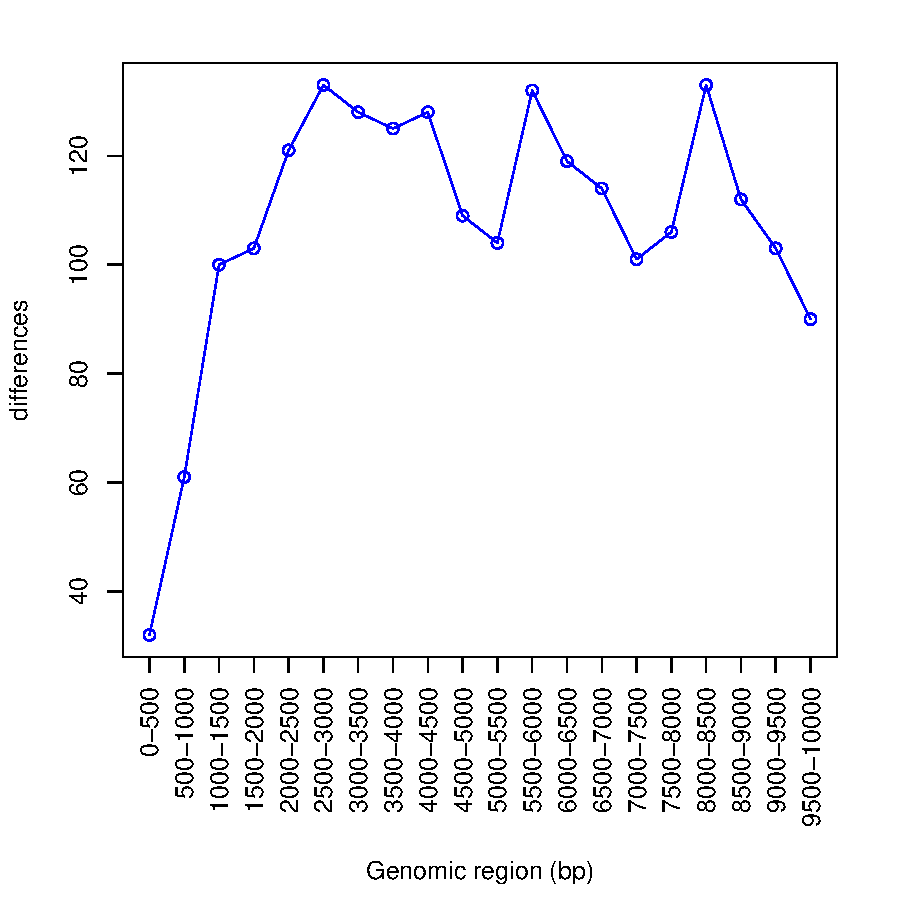
\includegraphics{geneXtendeR-038}
\end{center}
\end{figure}

This line plot is derived from the input peak dataset used from the H3K9me1 study examined earlier (Barbier et al. 2016).  If the study had examined a narrower chromatin mark (e.g., H3K4me3) then the decision process for choosing an optimal extension may have been different.  

In certain cases, additional extensions are unlikely to add significant value to the annotation of the peak file.  Taking the example of the 0-10000 bp line plot, an upstream extension beyond 3500 bp globally across every gene in a genome would most likely not accurately reflect the biology of the peak input file (since such large global upstream extensions are likely to reach considerably beyond known proximal promoter elements, especially for relatively narrow histone marks or transcription factors).  Such assumptions may be validated directly by the user by investigating the p-value and FDR of specific peaks using a combination of \texttt{HT-seq} (to count the reads) and \texttt{edgeR}/\texttt{DESeq2} (to assess statistical significance).  As such, \texttt{geneXtendeR} is designed to be used as part of a biological workflow involving subsequent statistical analysis:

\begin{figure}[H]
\centering
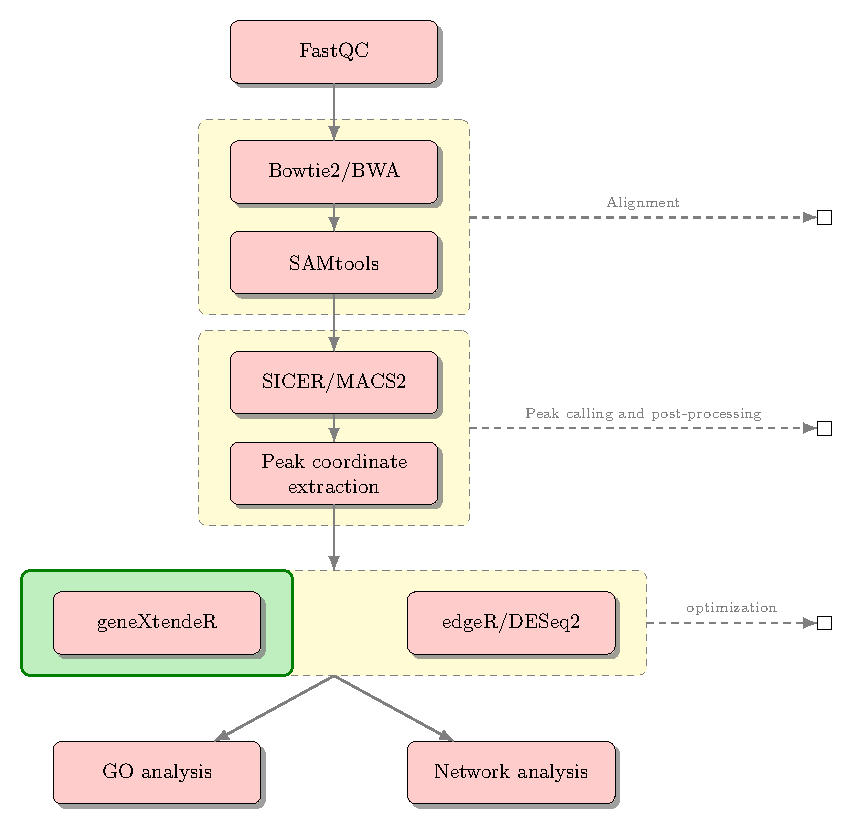
\includegraphics{figures/workflow.pdf}
\caption{Sample biological workflow using \texttt{geneXtendeR} in combination with existing statistical software to analyze peak significance.  Subsequent gene ontology enrichment or network analysis may be conducted on genes associated with statistically significant peaks.}
\end{figure}

It is entirely possible (and probable) for significant peaks to be present at relatively high upstream extension levels (i.e., large gene-spheres), albeit these significant peaks may be associated with biology not directly relevant to the study at-hand, due mainly to the sheer magnitude of the distance of the peak from traditional gene boundaries (where traditional gene boundaries may be loosely defined as +/- $\approx 3$ kb from TSS and +/- $\approx 0.5$kb from TES).  Consequently, it is likely for peaks-on-top-of-genes to exhibit higher levels of noise at higher upstream extension levels.  Nevertheless, this does not mean that potential enhancer activity should be discounted.  For instance, it is not uncommon to see a steady rise or even a surge in the number of peaks-on-top-of-genes at higher upstream extension levels:

\begin{figure}[H]
\begin{center}
\begin{Schunk}
\begin{Sinput}
> linePlot(rat, 7000, 8500, 100)
\end{Sinput}
\end{Schunk}
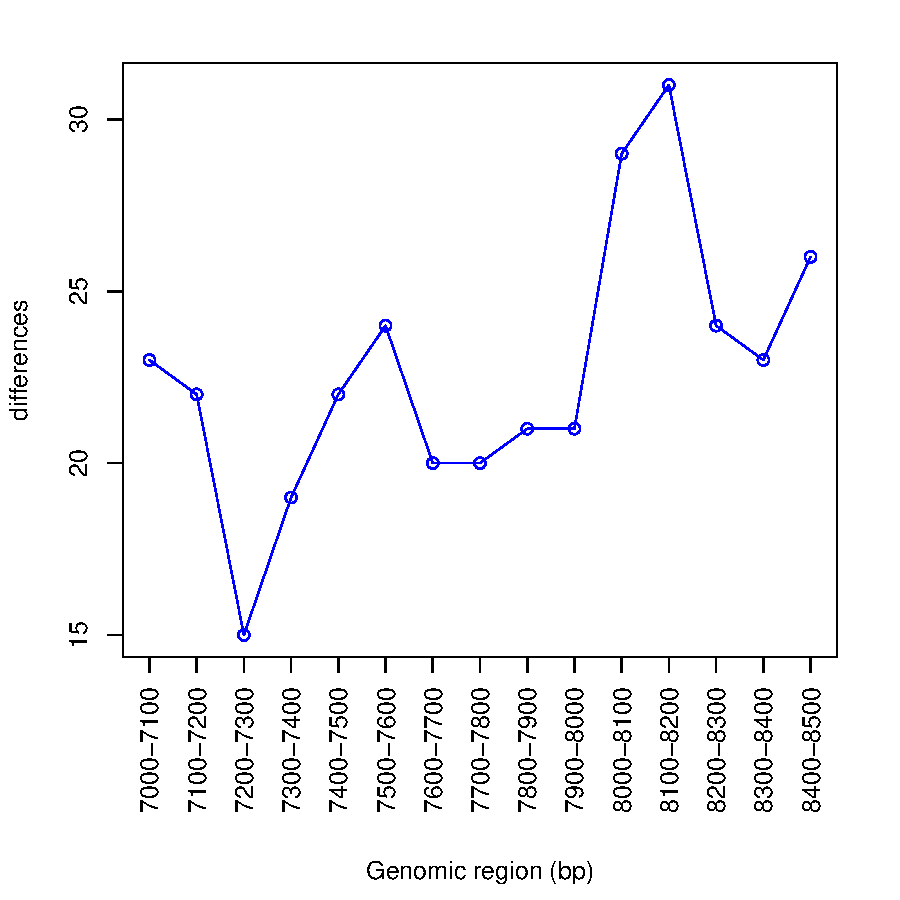
\includegraphics{geneXtendeR-039}
\end{center}
\end{figure}

This line plot shows that there are over 30 peaks in this dataset (across the rat genome) that reside between 8100 and 8200 bp upstream of their nearest gene.  In far-out cases like this, it is particularly recommended to examine the statistical significance of peaks to get a sense for the possibility of potential enhancer activity/regulation.  Of course, such computational findings would require experimental follow-up and/or database mining for known motifs.  Assessment of such statistical significance values is beyond the scope of \texttt{geneXtendeR}, in order to allow the user freedom to choose the most appropriate statistical package/technique for their analysis.  As before, first use the \texttt{distinct()} function to create a table of unique genes located under peaks between the two upstream extension levels:

%<<fig.width=6.2, fig.height=5>>=
\begin{Schunk}
\begin{Sinput}
> distinct(rat, 8100, 8200)
\end{Sinput}
\end{Schunk}

Then, assess the statistical significance of these peaks using a combination of \texttt{HT-seq} (Anders et al. 2015) and \texttt{edgeR} (Robinson et al. 2010), or \texttt{HT-seq} and \texttt{DESeq2} (Love et al. 2014), or some other appropriate combination of existing software tools.  Genes associated with the resultant statistically significant peaks may then be further assessed with gene ontology enrichment analysis to help answer a variety of interesting research questions.  It should once again be noted that the \texttt{diffGO()} function does NOT perform gene ontology enrichment analysis.  Instead, it returns all known gene ontologies for each gene.  The purpose and utility of this is described in the previous section.

Moreover, DNA sequences under peaks may be checked for the presence of known regulatory motifs (e.g., using \texttt{TRANSFAC} (Matys et al. 2006) or \texttt{MEME}/\texttt{JASPAR} (Sandelin et al. 2004, Bailey et al. 2009)), or for the presence of biological repeats (e.g., using \texttt{RepeatMasker} (Smit et al. 2015)). Pending a prospective GO enrichment and network analysis, functional validation may be followed up in the lab to test any potential regulatory sites or prospective enhancer elements, thereby bringing the computational analysis pipeline back to the bench.

In addition to the computational workflows discussed above, \texttt{geneXtendeR}'s wide array of functions makes it possible to conduct some rather interesting and creative combinations of genomic analysis.  Let's say, for example, that a user wants to explore all known ontological differences across specific disparate sectors of the genome (e.g., 0-500 bp vs. 2000-3000 bp, but removing 501-1999 bp from consideration).  In other words, look at all peaks (across the entire genome) that reside between 0-500 bp upstream of their nearest gene (and 2000-3000 bp upstream of their nearest gene), and extract unique gene ontologies that differ between these two variable-length sectors (where one is 500 bp long and the other is 1000 bp in length).  This can be accomplished rather conveniently using \texttt{dplyr}:

\begin{Schunk}
\begin{Sinput}
> library(dplyr)
> library(org.Rn.eg.db)
> library(GO.db)
> a <- diffGO(rat, 0, 500, BP, org.Rn.eg.db)
> b <- diffGO(rat, 2000, 3000, BP, org.Rn.eg.db)
> dplyr::filter(b, TERM %in% a$TERM)
\end{Sinput}
\begin{Soutput}
   gene$SYMBOL       GOID                                                TERM
1         Sod2 GO:0001889                                   liver development
2         Sod2 GO:0007507                                   heart development
3         Sod2 GO:0008285           negative regulation of cell proliferation
4         Sod2 GO:0042311                                        vasodilation
5         Sod2 GO:0042493                                    response to drug
6         Sod2 GO:0043066            negative regulation of apoptotic process
7         Dll1 GO:0001757                                somite specification
8         Dll1 GO:0008284           positive regulation of cell proliferation
9         Dll1 GO:0008285           negative regulation of cell proliferation
10        Dll1 GO:0045596         negative regulation of cell differentiation
11       Olr40 GO:0007186        G-protein coupled receptor signaling pathway
12      Olr139 GO:0007186        G-protein coupled receptor signaling pathway
13      Olr282 GO:0007186        G-protein coupled receptor signaling pathway
14      Gprc5b GO:0007186        G-protein coupled receptor signaling pathway
15        Aqp8 GO:0055085                             transmembrane transport
16        Aqp8 GO:0071320                           cellular response to cAMP
17    Cdc42bpg GO:0006468                             protein phosphorylation
18       Dusp5 GO:0045892 negative regulation of transcription, DNA-templated
19      Adgrl2 GO:0007166             cell surface receptor signaling pathway
20      Adgrl2 GO:0007186        G-protein coupled receptor signaling pathway
21      Nfe2l2 GO:0016567                              protein ubiquitination
22      Nfe2l2 GO:0071456                        cellular response to hypoxia
23      Olr559 GO:0007186        G-protein coupled receptor signaling pathway
24     Tspan18 GO:0007166             cell surface receptor signaling pathway
25       Kcnq2 GO:0060081                          membrane hyperpolarization
26       Reg3b GO:0008284           positive regulation of cell proliferation
27       Reg3b GO:0043066            negative regulation of apoptotic process
28      Olr828 GO:0007186        G-protein coupled receptor signaling pathway
29      Tspan9 GO:0007166             cell surface receptor signaling pathway
30     Bhlhe41 GO:0045892 negative regulation of transcription, DNA-templated
31        Aptx GO:0006974            cellular response to DNA damage stimulus
32       Ccl21 GO:0007186        G-protein coupled receptor signaling pathway
33       Aldob GO:0001889                                   liver development
34       Aldob GO:0042493                                    response to drug
35       Clic4 GO:1902476                    chloride transmembrane transport
36       Htr1d GO:0042310                                    vasoconstriction
37       Nlrc4 GO:0016567                              protein ubiquitination
38       Nlrc4 GO:0090307                            mitotic spindle assembly
39         Alk GO:0043066            negative regulation of apoptotic process
40       Esyt1 GO:0006869                                     lipid transport
41       Sbno2 GO:0045892 negative regulation of transcription, DNA-templated
42     Olr1085 GO:0007186        G-protein coupled receptor signaling pathway
43       Fbxo7 GO:0016567                              protein ubiquitination
44       Dnmt1 GO:0042493                                    response to drug
45       Dnmt1 GO:0045892 negative regulation of transcription, DNA-templated
46        Xcr1 GO:0007186        G-protein coupled receptor signaling pathway
47      Ccr1l1 GO:0007186        G-protein coupled receptor signaling pathway
48       Clcn7 GO:1902476                    chloride transmembrane transport
49   LOC684471 GO:0007186        G-protein coupled receptor signaling pathway
50         Il3 GO:0008284           positive regulation of cell proliferation
51         Il3 GO:0043066            negative regulation of apoptotic process
52     Olr1501 GO:0007186        G-protein coupled receptor signaling pathway
53       Socs3 GO:0016567                              protein ubiquitination
54       Socs3 GO:0042493                                    response to drug
55       Socs3 GO:0043066            negative regulation of apoptotic process
56       Fbxw8 GO:0016567                              protein ubiquitination
57      Fcgr2b GO:0007166             cell surface receptor signaling pathway
58    Arhgef10 GO:0090307                            mitotic spindle assembly
59      Eef1e1 GO:0008285           negative regulation of cell proliferation
60       F13a1 GO:0007596                                   blood coagulation
61       Tubb6 GO:0007010                           cytoskeleton organization
62     Csnk2a2 GO:0006468                             protein phosphorylation
63     Csnk2a2 GO:0051726                            regulation of cell cycle
64     Olr1735 GO:0007186        G-protein coupled receptor signaling pathway
\end{Soutput}
\begin{Sinput}
> 
\end{Sinput}
\end{Schunk}

This displays all biological process (BP) ontologies present in \texttt{b} that are not present in \texttt{a}.  Similarly, one can look at all BP, CC, or MF ontologies present in \texttt{a} that are not present in \texttt{b}. 

\section{Concluding remarks}

\texttt{geneXtendeR} is continually evolving, so any suggestions or new feature requests are always appreciated.  Likewise, any bug reports may be posted to \url{https://github.com/Bohdan-Khomtchouk/geneXtendeR/issues} or emailed to the package maintainer directly.    


\begin{thebibliography}{31}

\bibitem{anders}
Anders S, Pyl PT, Huber W:  \textit{HTSeq--a Python framework to work with high-throughput sequencing data.}  Bioinformatics.  2015, 31(2): 166--169. 

\bibitem{bailey}
Bailey TL, Boden M, Buske FA, Frith M, Grant CE, Clementi L, Ren J, Li WW, Noble WS:  \textit{MEME SUITE: tools for motif discovery and searching.}  Nucleic Acids Research.  2009, 37 (2): W202--W208. 

\bibitem{barbier}
Barbier E, Johnstone AL, Khomtchouk BB, Tapocik JD, Pitcairn C, Rehman F, Augier E, Borich A, Schank JR, Rienas CA, Van Booven DJ, Sun H, N\"{a}tt D, Wahlestedt C, Heilig M: \textit{Dependence-induced increase of alcohol self-administration and compulsive drinking mediated by the histone methyltransferase PRDM2}.  Molecular Psychiatry. 2016, Nature Publishing Group. doi: 10.1038/mp.2016.131.

\bibitem{gidlof}
Gidl\"{o}f, Johnstone AL, Bader K, Khomtchouk BB, et al.: \textit{Ischemic preconditioning confers epigenetic repression of Mtor and induction of autophagy through G9a-dependent H3K9 di-methylation.} Journal of the American Heart Association: Cardiovascular and Cerebrovascular Disease. 2016, 5(12): e004076.

\bibitem{heinz}
Heinz S, Benner C, Spann N, Bertolino E et al.: \textit{Simple Combinations of Lineage-Determining Transcription Factors Prime cis-Regulatory Elements Required for Macrophage and B Cell Identities.} Mol Cell 2010, 38(4): 576--589.

%\bibitem{khomtchouk}
%Khomtchouk BB, Van Booven DJ, Wahlestedt C: \textit{geneXtendeR: optimized functional annotation of ChIP-seq data}.  bioRxiv. 2016, 1--15. 

\bibitem{koohy}
Koohy H, Down TA, Spivakov M, Hubbard T: \textit{A Comparison of Peak Callers Used for DNase-Seq Data}.  PLoS One. 2014, 9(8): e105136. 

\bibitem{deseq2}
Love MI, Huber W, Anders S:  \textit{Moderated estimation of fold change and dispersion for RNA-seq data with DESeq2.}  Genome Biology.  2014, 15:550.

\bibitem{house}
House SL, Castro AM, Lupu TS, Weinheimer C, Smith C, Kovacs A, Ornitz DM: \textit{Endothelial fibroblast growth factor receptor signaling is required for vascular remodeling following cardiac ischemia-reperfusion injury.}  2016.  Am J Physiol Heart Circ Physiol.  310(5): H559--571.

\bibitem{matys}
Matys V, Kel-Margoulis OV, Fricke E, Liebich I, Land S, Barre-Dirrie A, Reuter I, Chekmenev D, Krull M, Hornischer K, Voss N, Stegmaier P, Lewicki-Potapov B, Saxel H, Kel AE, Wingender E:  \textit{TRANSFAC and its module TRANSCompel: transcriptional gene regulation in eukaryotes.}  2006.  Nucleic Acids Research.  34 (Database issue): D108--110.

\bibitem{ong}
Ong W, Ng MP, Loke S, Jin S, Wu Y, Tanaka K, Wong T: \textit{Comprehensive Gene Expression Profiling Reveals Synergistic Functional Networks in Cerebral Vessels after Hypertension or Hypercholesterolemia.}  2013.  PLoS One.  8(7): e68335.

\bibitem{quinlan}
Quinlan AR, Hall IM: \textit{BEDTools: a flexible suite of utilities for comparing genomic features}. Bioinformatics. 2010, 26(6): 841--842.

\bibitem{edgeR}
Robinson MD, McCarthy DJ, Smyth GK: \textit{edgeR: a Bioconductor package for differential expression analysis of digital gene expression data}. Bioinformatics. 2010, 26: 139--140.

\bibitem{sandelin}
Sandelin A, Alkema W, Engstrom P, Wasserman WW, Lenhard B:  \textit{JASPAR: an open-access database for eukaryotic transcription factor binding profiles.}  Nucleic Acids Research.  2004, 32 (Database issue): D91--D94.  

\bibitem{smit}
Smit AFA, Hubley R, Green P. RepeatMasker Open-4.0.  2013-2015  \url{<http://www.repeatmasker.org>}.

\bibitem{thomas}
Thomas R, Thomas S, Holloway AK, Pollard KS: \textit{Features that define the best ChIP-seq peak calling algorithms}.  Briefings in Bioinformatics.  2017, 18(3): 441--450.

\bibitem{zang}
Zang C, Schones DE, Zeng C, Cui K, Zhao K, Peng W:  \textit{A clustering approach for identification of enriched domains from histone modification ChIP-Seq data.}  Bioinformatics.  2009, 25(15): 1952--1958.

\bibitem{zhang}
Zhang Y, Liu T, Meyer CA, Eeckhoute J, Johnson DS, Bernstein BE, Nusbaum C, Myers RM, Brown M, Li W, Liu XS:  \textit{Model-based analysis of ChIP-Seq (MACS).}  Genome Biology.  2008, 9(9): R137.

\bibitem{zhu}
Zhu L, Gazin C, Lawson N, Pages H, Lin S, Lapointe D, Green M: \textit{ChIPpeakAnno: a Bioconductor package to annotate ChIP-seq and ChIP-chip data}.  BMC Bioinformatics.  2010, 11(1), pp. 237.

\end{thebibliography}


\end{document}
